%%%%%%%%%%%%%%%%%%%%%%%%%%%%%%%%%%%%%%%%%%%%%%%%%%%%%%%%%%%%%%%%%%%%%%%%%%%%%%%%%%%%%%%%%%%%%%%%%
% Chapter 5: Results   (the \chapter command is in main.tex)
%
% One section per block of work. Figures for each project day go in figures/ with a dayN_ prefix
% (e.g. figures/day3_soc_e1.png). Only numbers from actual runs go in this chapter.
%%%%%%%%%%%%%%%%%%%%%%%%%%%%%%%%%%%%%%%%%%%%%%%%%%%%%%%%%%%%%%%%%%%%%%%%%%%%%%%%%%%%%%%%%%%%%%%%%

This chapter first checks that the simulator behaves as intended (Section~\ref{sec:r_sim}). It then presents the estimation experiments E1--E8 (Section~\ref{sec:r_estimation}), the decisions of the four policies on one flight (Section~\ref{sec:r_single_rth}), the Monte Carlo comparison (Section~\ref{sec:r_mc}) and the risk-threshold sweep (Section~\ref{sec:r_sweep}).

%--------------------------------------------------------------------------------------------------
\section{Simulator verification}\label{sec:r_sim}
%--------------------------------------------------------------------------------------------------

Before any filter is added, the simulator must produce believable data: the voltage should sag under load, change in the right direction at each phase change, and stay above the cut-off on a mission that is meant to be safe. This section reports one test flight made with \texttt{main\_day2\_simulator.m} (Section~\ref{sec:i_loop}).

\subsection{Set-up}

The drone flew the \emph{short} mission (three drop-offs, Section~\ref{sec:m_mission}) with no wind. The true battery started at rest at 95\% SoC and used the true parameters of Table~\ref{tab:m_params}, except that the slow RC pair was at its first setting, $R_2 = 4$\,m$\Omega$ and $C_2 = 100\,000$\,F. This setting was later kept only for the E6 stress test (Section~\ref{sec:m_why_mismatch}). The current sensor had a bias of $+0.5$\,A and noise of 0.2\,A; the voltage sensor had noise of 10\,mV. The random seed was fixed (\texttt{rng(2)}). No estimator was running; charge counting was applied to the logged measured current after the flight. Table~\ref{tab:r_day2} summarises the flight.

\begin{table}[htbp]
  \centering
  \caption{Simulator test flight: summary (short mission, one run).}
  \label{tab:r_day2}
  \begin{tabular}{@{}ll@{}}
    \toprule
    Quantity & Value \\
    \midrule
    Outcome & Landed safely \\
    Flight time & 14.2\,min \\
    Distance flown & 6.89\,km \\
    True SoC, start $\rightarrow$ landing & 95\% $\rightarrow$ 18.5\% \\
    Lowest cell voltage & 3.297\,V (cut-off 3.0\,V) \\
    Largest voltage sag (OCV $-$ terminal voltage) & 367\,mV per cell, at take-off (30\,A) \\
    Charge-counting SoC error at landing & $-2.3\%$ \\
    \bottomrule
  \end{tabular}
\end{table}

\subsection{OCV curve}

Figure~\ref{fig:r_ocv} shows the OCV curve that the filter believes and the true battery's curve, 5\,mV lower. The two are almost indistinguishable by eye, yet 5\,mV corresponds to about 1\% SoC in the flat middle of the curve, so even this small offset is a real test for the filter. The right-hand axis shows the slope that becomes the first entry of $H$ in \eqref{eq:m_F}. It is several times larger near empty than in the middle, so the voltage corrects the SoC much more strongly at low charge.

\begin{figure}[htbp]
  \centering
  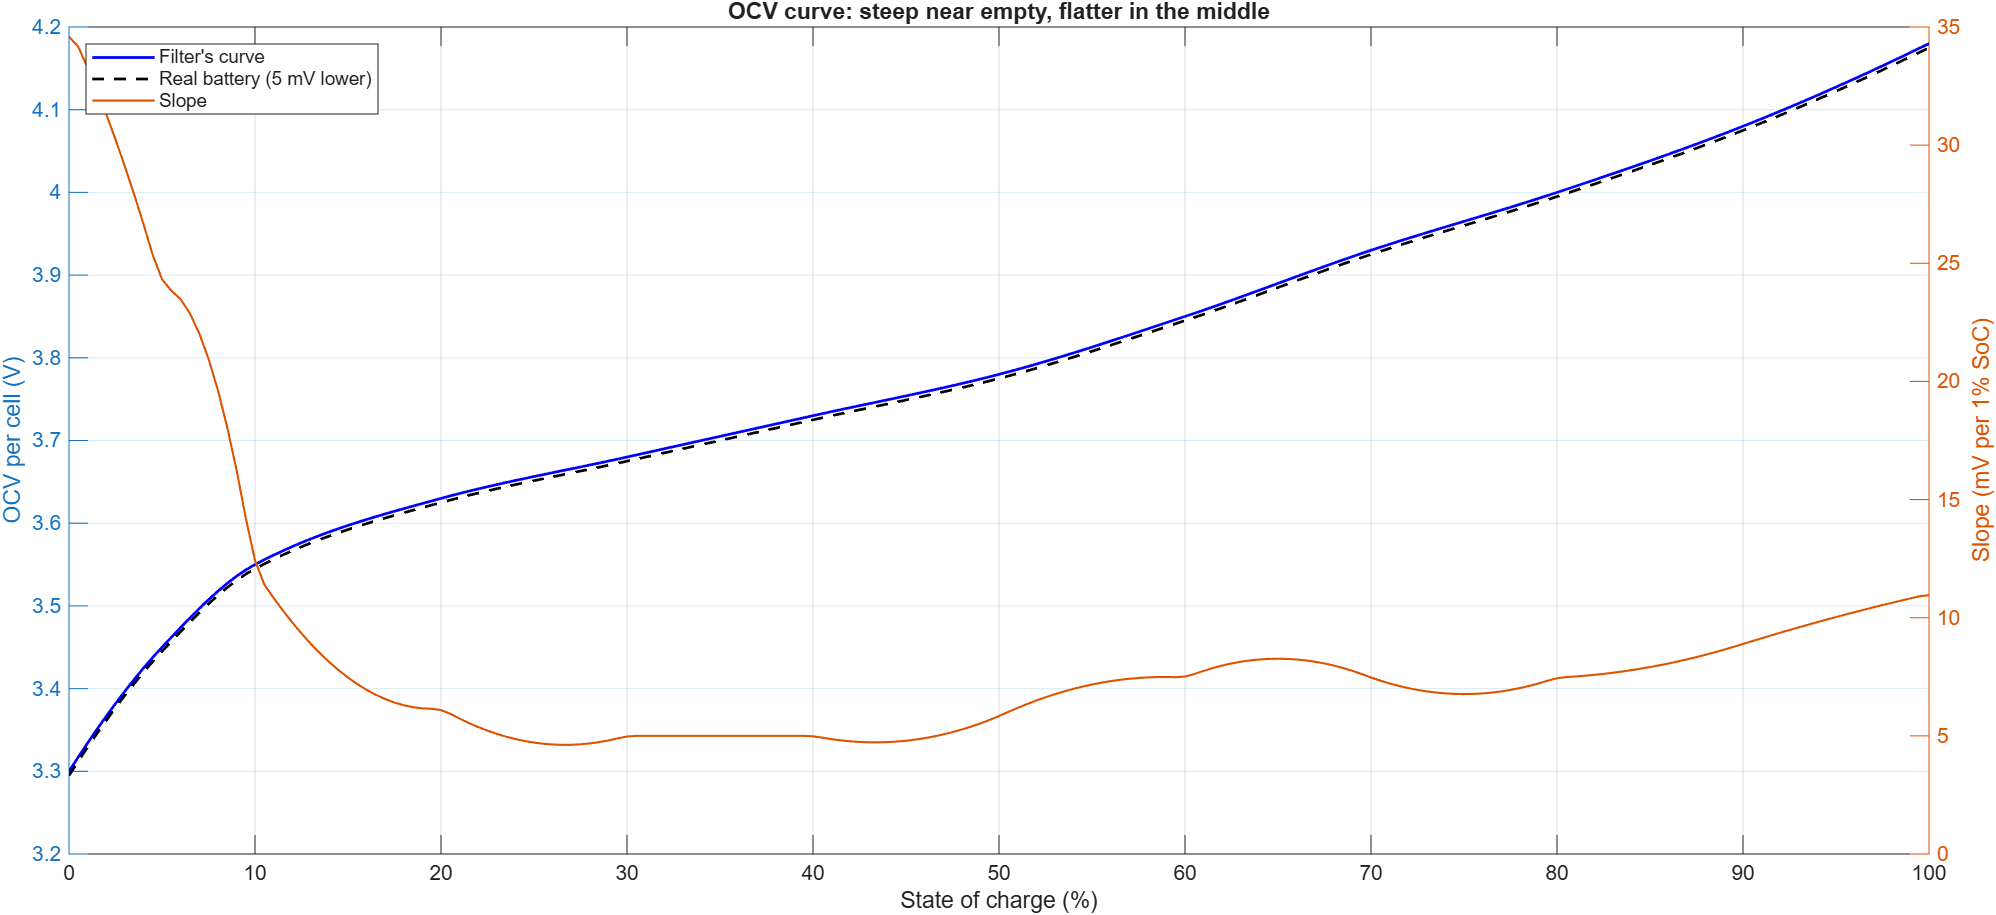
\includegraphics[width=\textwidth]{day2_ocv_curve.png}
  \caption{OCV curve of the filter (solid) and of the true battery (dashed, 5\,mV lower), with the slope $d\,\mathrm{OCV}/d\,\mathrm{SoC}$ on the right axis. Notice that the slope, which sets how much the voltage can tell the EKF about the SoC, is high below about 10\% SoC and low between about 20\% and 50\%.}
  \label{fig:r_ocv}
\end{figure}

\subsection{Mission and current}

Figure~\ref{fig:r_mission} shows the flight path and the current. Two simple checks confirm that the drone model works. First, the straight legs home $\rightarrow$ drop~1 $\rightarrow$ drop~2 $\rightarrow$ drop~3 $\rightarrow$ home add up to 6.89\,km, the same as the logged distance flown, so the drone neither overshoots its targets nor cuts corners. Second, 6.89\,km at 10\,m/s takes about 689\,s; adding 30\,s of take-off, three 30\,s hovers and 40\,s of landing gives about 849\,s, or 14.2\,min, which matches the logged flight time.

The current profile shows each phase clearly: 30\,A at take-off, about 15\,A in cruise, three 20\,A blocks while hovering at the drop-offs, and 18\,A while landing. The slow random load of \eqref{eq:m_wobble} makes the current wander slowly, by about 0.7\,A (one standard deviation). The measured current (grey) sits slightly above the true current (blue), because of the $+0.5$\,A bias, and is noisier.

\begin{figure}[htbp]
  \centering
  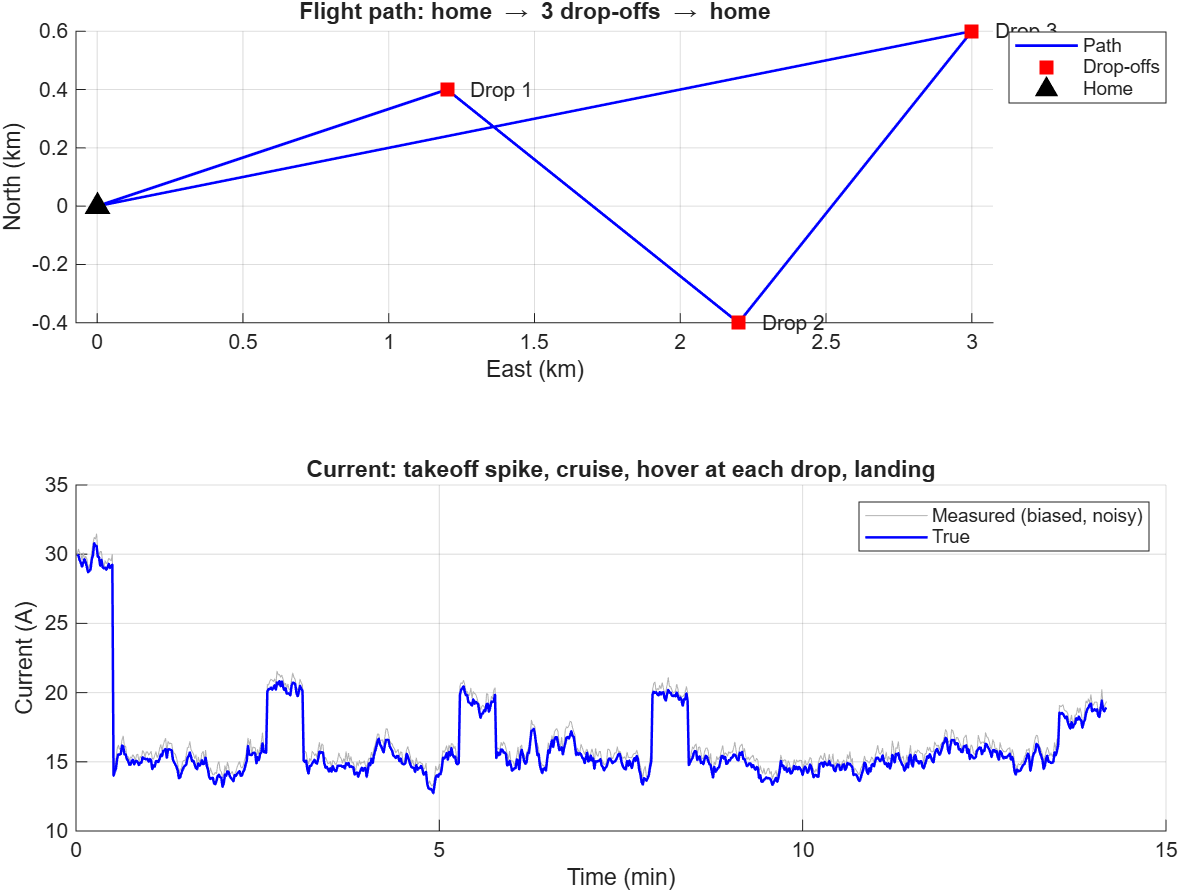
\includegraphics[width=\textwidth]{day2_mission.png}
  \caption{Simulator test flight. Top: flight path from home through three drop-offs and back. Bottom: true current (blue) and measured current (grey). Notice the take-off spike, the three hover blocks and the landing phase, and that the measured current runs slightly above the truth because of the sensor bias.}
  \label{fig:r_mission}
\end{figure}

\subsection{Voltage and state of charge}

Figure~\ref{fig:r_voltage} shows the voltages and the true SoC. The true SoC falls from 95\% to 18.5\%, steadily in cruise and slightly faster during take-off and hover, when the current is higher.

\textbf{Voltage sag.} The gap between the OCV (dashed) and the terminal voltage (blue) is the sag. It is largest at take-off, 367\,mV per cell at 30\,A. Of this, the ohmic part alone \eqref{eq:bg_sag} is $R_0 I = 8.8\text{\,m}\Omega \times 30\text{\,A} = 264$\,mV; the rest is polarisation that builds up in the RC pairs during the 30\,s climb. A simple voltage gauge would therefore read the battery as much emptier than it is during take-off.

\textbf{Steps at phase changes.} When take-off ends and the current falls from 30\,A to 15\,A, the voltage steps \emph{up}; at each drop-off, when the current rises to 20\,A for hovering, it steps \emph{down}. The instant part of each step is $R_0 \Delta I$, about 132\,mV when take-off ends and 44\,mV at the start of each hover, and the rounded part that follows is the RC voltage settling. This is the behaviour the circuit model of Figure~\ref{fig:bg_circuit} predicts.

\textbf{Slowly widening gap.} Over the flight, the gap between the OCV and the terminal voltage slowly widens, even in cruise at a nearly constant current. This is the slow RC pair ($\tau_2 = 400$\,s), which exists only in the true battery and keeps charging up for most of the flight. It is the deliberate model mismatch of Section~\ref{sec:m_why_mismatch}: the EKF, with its single 30\,s RC pair, cannot represent this slow drift and has to absorb it in its other states. This observation, together with a rough estimate of the settled extra drop, led to a milder default slow pair for the main experiments, with the original setting kept as the E6 stress test.

\textbf{Safety.} The lowest cell voltage, 3.297\,V near the end of the flight, stays about 0.3\,V above the 3.0\,V cut-off, and the drone landed with 18.5\% SoC. The short mission is therefore safe, as intended, and leaves the long mission to test the RTH rule.

The figure also hints at the weakness of policy A (Table~\ref{tab:m_policies}). The measured voltage first stayed below 3.6\,V (the threshold first planned for policy A) for 5 consecutive seconds at 5.4\,min, during the hover at the second drop-off, when the true SoC was still 64.9\%. A voltage-threshold rule at that level would have turned back with most of the battery unused. This is one reason the final policy A uses 3.5\,V and is swept over a range of thresholds (Section~\ref{sec:m_policies}).

\begin{figure}[htbp]
  \centering
  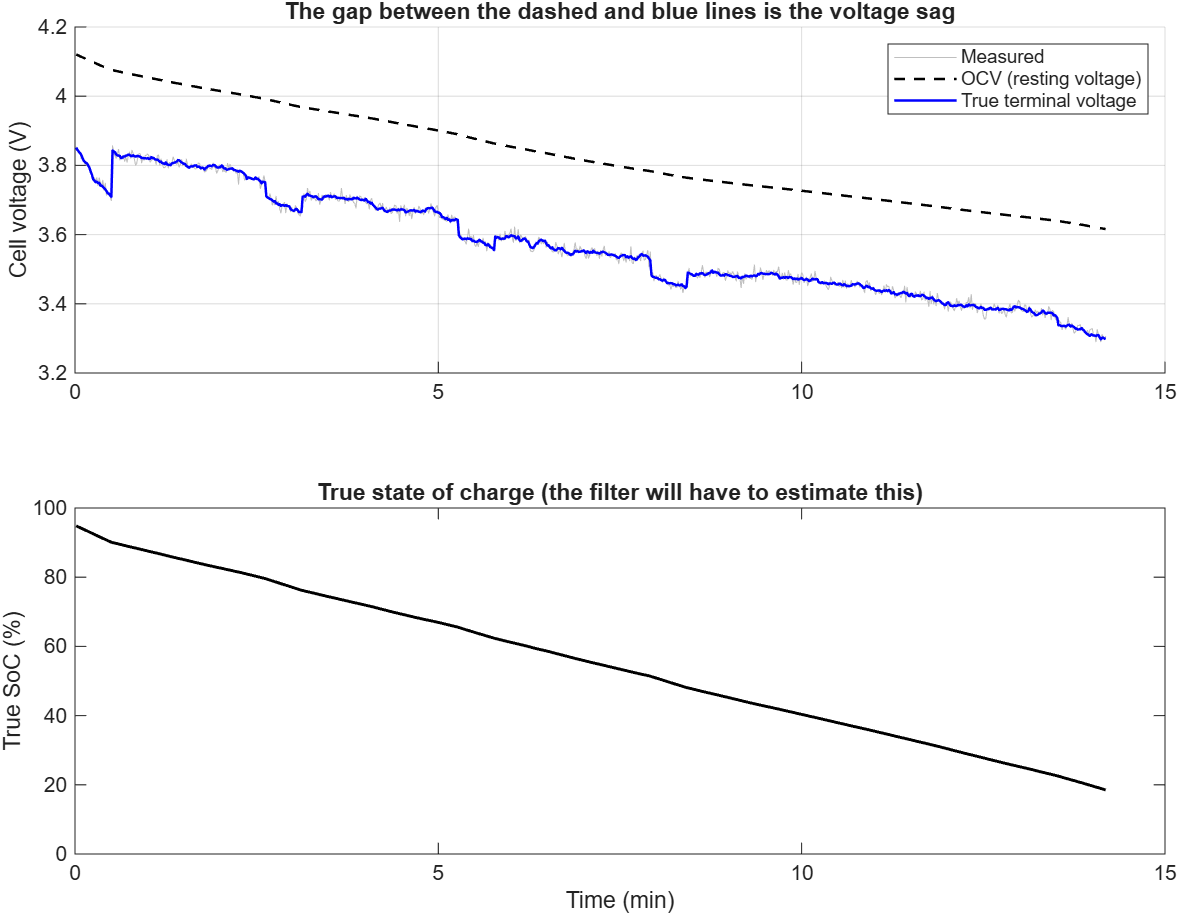
\includegraphics[width=\textwidth]{day2_voltage_soc.png}
  \caption{Simulator test flight. Top: OCV (dashed), true terminal voltage (blue) and measured voltage (grey), per cell. Bottom: true SoC. Notice the large sag at take-off, the step up when take-off ends, the steps down during each hover, and the gap that slowly widens through the flight because of the slow RC pair that only the true battery has.}
  \label{fig:r_voltage}
\end{figure}

\subsection{Charge counting with a biased sensor}

Charge counting \eqref{eq:bg_cc}, applied to the measured current, ended the flight 2.3\% below the true SoC. Equation~\eqref{eq:bg_cc_drift} predicts this: a 0.5\,A bias over 14.2\,min removes about 0.118\,Ah, or about 2.4\% of 5\,Ah. The sign is negative because the sensor reads too high, so the counter believes more charge has been used than really has. The small difference from 2.4\% is due to the sensor noise. This drift grows linearly with time and would be larger on a longer flight or with a larger bias, and it is one of the errors the EKF is designed to remove.

\subsection{Summary of the simulator check}

The simulator behaves as intended. The voltage sags realistically under load, it steps in the correct direction at every phase change, the drone's distance and flight time agree with the route, the charge-counting drift matches theory, and the deliberate mismatch between the true battery and the filter's model is visible in the data. This check is based on a single run with one random seed; it verifies behaviour, not statistics.

%--------------------------------------------------------------------------------------------------
\section{Estimation experiments}\label{sec:r_estimation}
%--------------------------------------------------------------------------------------------------

Experiments E1 and E2 were run with \texttt{main\_day3\_ekf.m} (Section~\ref{sec:i_run_flight}) on the short mission, with the default true battery of Table~\ref{tab:m_params} (slow pair $R_2 = 1.5$\,m$\Omega$), the sensor errors of Section~\ref{sec:m_sensors} (current bias $+0.5$\,A) and random seed~2. Three estimators were compared on exactly the same sensor readings: charge counting, EKF stage~A (learns SoC and $V_1$) and EKF stage~B (also learns $R_0$). Both EKF stages used the model-error allowance $\sigma_{\text{model}} = 10$\,mV. Table~\ref{tab:r_e1e2} summarises the results. The convergence time is the last time the SoC error was 2\% or more; ``never'' means the error was still at least 2\% at landing.

\begin{table}[htbp]
  \centering
  \caption[SoC estimation in E1 and E2.]{SoC estimation in E1 and E2 (MATLAB, short mission, seed 2). Errors are estimate minus truth, in percentage points of SoC. Final: error at landing. Max: largest absolute error. In $\pm 3\sigma$: share of time the truth was inside the EKF's band. NIS: mean NIS. $<2\%$ after: time after which the error stayed below 2\%.}
  \label{tab:r_e1e2}
  \small
  \setlength{\tabcolsep}{4pt}
  \begin{tabular}{@{}llcccccc@{}}
    \toprule
    & Estimator & RMSE & Final & Max & In $\pm 3\sigma$ & NIS & $<2\%$ after \\
    \midrule
    E1 & Charge counting & 4.36\% & $-5.50\%$ & 5.50\% & -- & -- & -- \\
       & EKF stage A     & 2.51\% & $-3.89\%$ & 3.90\% & 17\%  & 0.54 & never \\
       & EKF stage B     & 0.97\% & $-1.53\%$ & 3.76\% & 100\% & 0.51 & 30\,s \\
    \midrule
    E2 & Charge counting & 13.85\% & $+12.64\%$ & 15.00\% & -- & -- & -- \\
       & EKF stage A     & 2.49\% & $-2.49\%$ & 3.62\% & 18\%  & 0.60 & never \\
       & EKF stage B     & 1.32\% & $-0.38\%$ & 7.52\% & 100\% & 0.51 & 42\,s \\
    \bottomrule
  \end{tabular}
\end{table}

\begin{figure}[htbp]
  \centering
  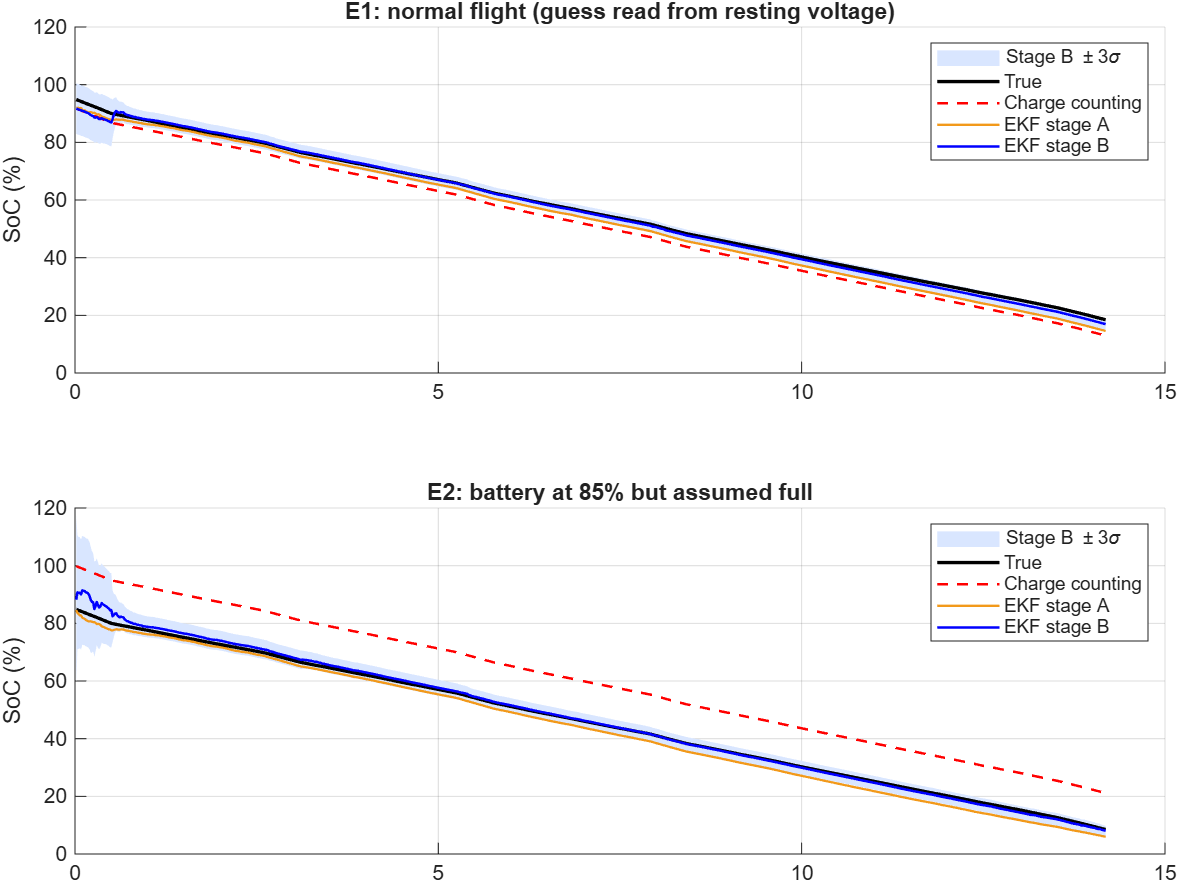
\includegraphics[width=\textwidth]{day3_soc_tracking.png}
  \caption{SoC estimates in E1 (top) and E2 (bottom): truth (black), charge counting (red dashed), EKF stage A (orange) and stage B (blue) with its $\pm 3\sigma$ band. Notice that stage B stays on the true SoC in both flights, while charge counting keeps its starting error, and in E2 believes the battery holds about 21\% at landing when it really holds about 9\%.}
  \label{fig:r_soc_tracking}
\end{figure}

\begin{figure}[htbp]
  \centering
  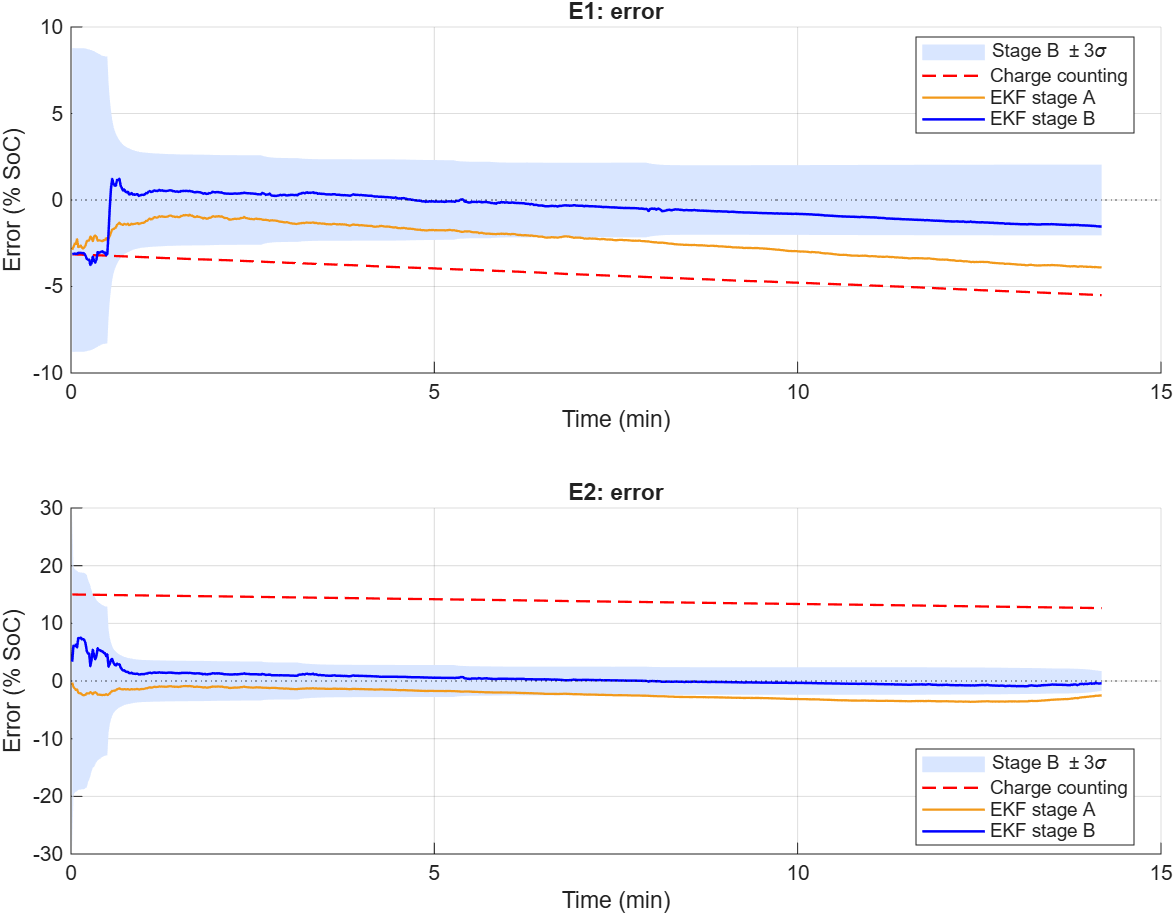
\includegraphics[width=\textwidth]{day3_soc_error.png}
  \caption{SoC error (estimate minus truth) in E1 (top) and E2 (bottom), with the stage-B $\pm 3\sigma$ band. Notice the jump in the stage-B error and the collapse of its band at about 0.5\,min, when take-off ends; after that, the stage-B error stays inside its band, while stage A drifts steadily below it and charge counting drifts linearly.}
  \label{fig:r_soc_error}
\end{figure}

\subsection{E1: Nominal flight}\label{sec:r_e1}

\textbf{Starting guess.} The true battery started at 95\%. The SoC read from the resting voltage before take-off was about 92\%, roughly 3\% low. Near full charge the OCV curve rises by about 10\,mV per 1\% SoC (Figure~\ref{fig:bg_ocv_tangent}, 90--100\%), so the $-5$\,mV offset of the true curve accounts for about 0.5\% of this, and the rest comes from the noise on the single voltage reading (10\,mV, about 1\% SoC per standard deviation). All three estimators started from this guess.

\textbf{Charge counting} never corrects the start error and adds the drift caused by the sensor bias. Its error grows linearly from about $-3\%$ to $-5.50\%$ at landing (Figure~\ref{fig:r_soc_error}). The growth matches \eqref{eq:bg_cc_drift}: a $+0.5$\,A bias over about 14\,minutes adds about $-2.4\%$.

\textbf{Stage A} (no $R_0$ state) first moves towards the truth, but then drifts steadily low. It ends at $-3.89\%$ and spends most of the flight outside the stage-B band. Its own $\pm 3\sigma$ band contained the truth only 17\% of the time: the filter is both biased and overconfident. This is the behaviour the design-stage investigation predicted (Section~\ref{sec:m_ekf_investigation}): the true $R_0$ is 10\% higher than the filter assumes, and stage~A can only explain the extra sag as a lower SoC.

Stage~A's mean NIS of 0.54 looks healthy, and this is itself a lesson. Stage~A explains the measured voltage well, but with the wrong SoC, so its innovations stay small. The innovation-based checks only see whether the voltage is explained, not whether the hidden state is right. Only a comparison with the truth (NEES, or the $\pm 3\sigma$ check above) reveals the bias, and that is possible only in simulation.

\textbf{Stage B} ends at $-1.53\%$ with an RMSE of 0.97\%, less than a quarter of the charge-counting RMSE and less than half that of stage~A. Its $\pm 3\sigma$ band contained the truth 100\% of the time.

\textbf{The take-off current step.} The most instructive moment of the flight is at about 0.5\,min, when take-off ends and the current steps from 30\,A to 15\,A. At that moment three things happen together (Figures~\ref{fig:r_soc_error} and~\ref{fig:r_r0}):
\begin{itemize}
  \item the stage-B SoC error jumps from about $-3\%$ to about $+1\%$;
  \item its $\pm 3\sigma$ band collapses from about $\pm 8.5\%$ to about $\pm 2.5\%$;
  \item the $R_0$ estimate jumps from about 7.7--8.0\,m$\Omega$ to about 8.9\,m$\Omega$.
\end{itemize}
During take-off the current is almost constant at 30\,A. A voltage that is lower than expected can then be explained equally well by a lower SoC or by a higher $R_0$, so the two cannot be separated, and the filter keeps both uncertain. The measurement Jacobian \eqref{eq:m_F} shows why the current step resolves this. The SoC entry, $d\,\mathrm{OCV}/d\,\mathrm{SoC}$, does not depend on the current, but the $R_0$ entry, $-(I_m - \hat{b})$, halves when the current halves. Only when the current changes does the voltage carry separate information about the two states. The current step provides this \emph{excitation}: the instant voltage jump it causes has the size $R_0\,\Delta I$, which pins down $R_0$, and with $R_0$ known the remaining voltage level pins down the SoC. This is the observability argument of Section~\ref{sec:m_ekf_investigation} seen in a real run, and it is why the stage-B error falls below 2\% exactly 30\,s into the flight, when take-off ends.

\begin{figure}[htbp]
  \centering
  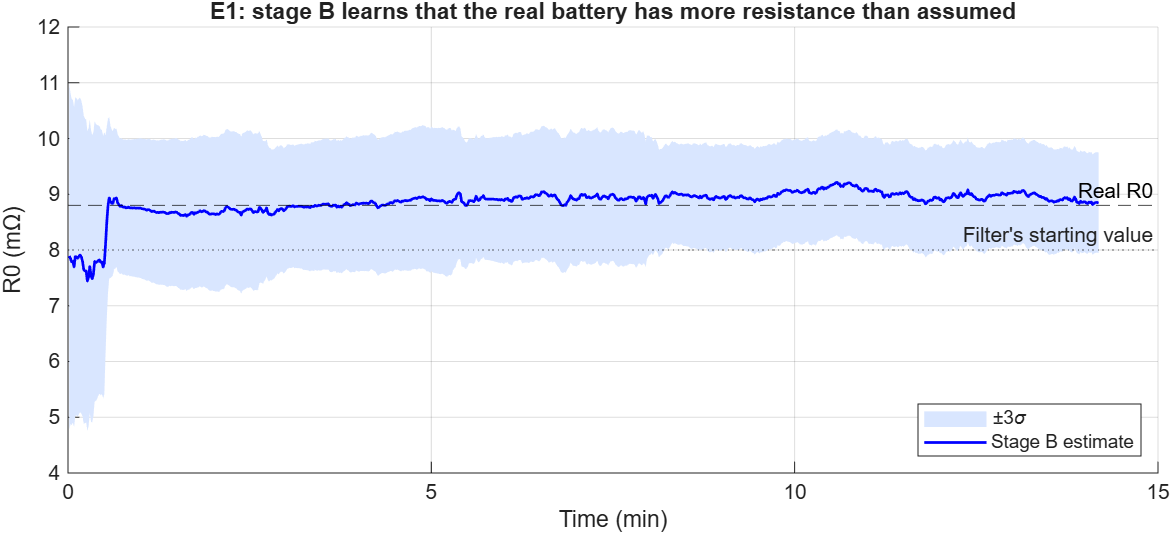
\includegraphics[width=\textwidth]{day3_r0_estimate.png}
  \caption{Stage-B estimate of $R_0$ in E1, with its $\pm 3\sigma$ band. Notice that the estimate barely moves during the constant-current take-off, then jumps to the true value (8.8\,m$\Omega$) when the current steps down at about 0.5\,min, and that the band always contains the true value.}
  \label{fig:r_r0}
\end{figure}

\textbf{Resistance estimate.} After the step the $R_0$ estimate settles between about 8.8 and 9.1\,m$\Omega$ and ends the flight at 8.85\,m$\Omega$, against a true value of 8.8\,m$\Omega$ and a starting value of 8.0\,m$\Omega$. Its $\pm 3\sigma$ band, about $\pm 1$\,m$\Omega$ wide, always contains the true value.

\textbf{Is the filter honest?} Figure~\ref{fig:r_e1_innov} compares the measured voltage with the voltage stage~B expected before each update. The expected voltage follows every sag and step. The innovations look like white noise around zero and stay well inside $\pm 3\sqrt{S_k}$ after the first few seconds; the band is wide only at the very start because of the large initial uncertainty. The mean NIS of 0.51 is below 1, so the filter is slightly more cautious than necessary. This is the expected effect of the 10\,mV model-error allowance, chosen on purpose to keep the bands honest (Section~\ref{sec:m_ekf_investigation}).

\begin{figure}[htbp]
  \centering
  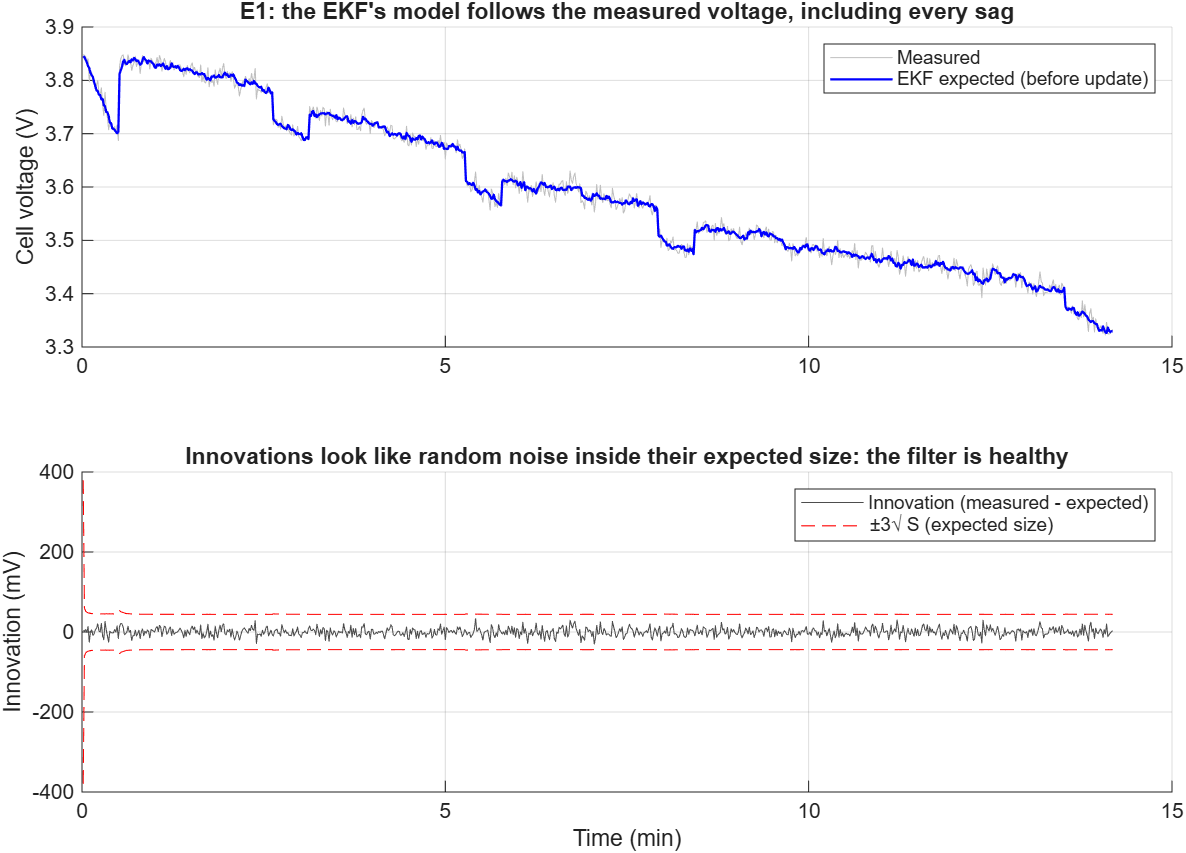
\includegraphics[width=\textwidth]{day3_e1_voltage_innovation.png}
  \caption{E1, stage B. Top: measured cell voltage (grey) and the voltage the EKF expected before each update (blue). Bottom: innovations with their expected size $\pm 3\sqrt{S}$. Notice that the model follows every sag and step, and that the innovations look like zero-mean noise well inside the band after the first seconds.}
  \label{fig:r_e1_innov}
\end{figure}

\textbf{Remaining error.} Stage~B still drifts slowly low during the flight and ends at $-1.53\%$. The most likely cause is the slow RC pair ($R_2 = 1.5$\,m$\Omega$, $\tau_2 = 400$\,s), which only the true battery has and which builds up over the flight (Section~\ref{sec:m_why_mismatch}). The filter has no state for it, so part of the extra drop is read as a lower SoC. The error stays inside the $\pm 3\sigma$ band, so the filter's stated uncertainty remains honest; this is discussed further in Section~\ref{sec:d_mismatch}.

\subsection{E2: Wrong initial SoC}\label{sec:r_e2}

In E2 the true battery started at 85\%, but all three estimators assumed a full battery (100\%). The EKF was told that this guess was uncertain ($\sigma_{\text{SoC},0} = 20\%$).

\textbf{Charge counting} keeps the $+15\%$ start error for the whole flight, reduced slowly by the bias drift, and ends $+12.64\%$ high. The consequence is serious. At landing the true SoC is only about 9\% (8.6\%), below the 10\% reserve, while charge counting believes the battery still holds about 21\%. A drone relying on charge counting would land nearly empty while believing it had a fifth of its battery left. On a longer route it would have flown on past the point of no return. This is exactly the failure the risk-aware RTH rule is designed to prevent.

\textbf{Stage B} starts at 100\% with a wide band. For the first 30\,s, during take-off, it sits about 5--7\% too high (maximum error 7.52\%). Then, at the take-off current step, it converges: within about 1\% of the truth by about 1\,min, and with the error staying below 2\% after 42\,s. For the rest of the flight it stays close to the truth and ends at $-0.38\%$, inside its band 100\% of the time. The slow start has the same cause as in E1. While the current is constant, a voltage that is lower than a full battery would give can be explained partly by a higher $R_0$ instead of a lower SoC, so stage~B cannot fully correct the SoC until the current step separates the two.

\textbf{Stage A} has no $R_0$ state, so it has no such ambiguity and corrects the start error within the first seconds. But it then drifts low for the same reason as in E1, ends at $-2.49\%$, and contains the truth in its band only 18\% of the time. Its ``never'' in Table~\ref{tab:r_e1e2} reflects this late drift, not a failure to recover from the wrong start.

\subsection{Comparison with the design-stage checks}\label{sec:r_e1e2_python}

The MATLAB results show the same pattern as the design-stage checks in the Python port (Section~\ref{sec:m_ekf_investigation}). For stage~B, the SoC RMSE was 0.97\% in MATLAB against 1.04\% in the port for E1, and 1.32\% against 1.00\% for E2. The two implementations use different random-number generators, so the same seed gives different noise, and single-run numbers differ slightly. The largest difference is for charge counting in E1 (4.36\% in MATLAB against 1.60\% in the port). This is because the MATLAB resting-voltage guess happened to be about 3\% low, and charge counting never corrects a start error. The 20-flight averages of E8 (Section~\ref{sec:r_e8}) remove this single-run luck.

\subsection{Common settings for E3 to E8}\label{sec:r_day4_setup}

Experiments E3--E8 were run with \texttt{main\_day4\_experiments.m} (Section~\ref{sec:i_day4}) on the short mission. The starting SoC was read from 10 averaged resting readings, and single runs used seed~2. Because of the averaging, the random numbers differ from the first E1 and E2 runs, so the E1 and E2 scenarios inside E8 do not reproduce Table~\ref{tab:r_e1e2} exactly. Besides the errors, the tables give the mean NEES on the SoC ($e^2/P_{11}$, Section~\ref{sec:m_ekf_consistency}), which should be about 1 for an honest filter; much larger means overconfident.

\subsection{E3: Bias observability (stage C)}\label{sec:r_e3}

In E3 the current sensor read 0.8\,A too high instead of 0.5\,A. Table~\ref{tab:r_e3e4} and Figure~\ref{fig:r_e3} show the results.

\begin{table}[htbp]
  \centering
  \caption[Single runs of E3 and E4.]{Single runs of E3 (bias 0.8\,A) and E4 (aged battery), seed 2. NEES is the mean NEES on the SoC (about 1 for an honest filter).}
  \label{tab:r_e3e4}
  \small
  \begin{tabular}{@{}llccccc@{}}
    \toprule
    & Estimator & RMSE & Final error & Inside $\pm 3\sigma$ & Mean NIS & Mean NEES \\
    \midrule
    E3 & Charge counting & 3.13\% & $-4.83\%$ & -- & -- & -- \\
       & EKF stage B     & 1.28\% & $-2.50\%$ & 88\%  & 0.51 & 3.10 \\
       & EKF stage C     & 1.58\% & $-1.88\%$ & 100\% & 0.51 & 0.64 \\
    \midrule
    E4 & Charge counting & 5.72\% & $+10.20\%$ & -- & -- & -- \\
       & EKF stage B     & 4.64\% & $+8.47\%$ & 28\%  & 0.56 & 44.81 \\
       & EKF stage C     & 0.80\% & $+0.17\%$ & 100\% & 0.51 & 0.22 \\
    \bottomrule
  \end{tabular}
\end{table}

\textbf{Charge counting} drifts low at a steady rate and ends at $-4.83\%$. This matches \eqref{eq:bg_cc_drift}: 0.8\,A for about 14\,minutes is about 0.19\,Ah, or 3.8\% of 5\,Ah, on top of a start error of about $-1\%$.

\textbf{Both EKF stages} do much better. Stage~B, which does not model the bias, is slightly more accurate (RMSE 1.28\%), because the voltage keeps correcting the drift the bias causes. Its band, however, contained the truth only 88\% of the time, and its mean NEES of 3.10 shows it is overconfident: it does not know about the extra error. Stage~C ended closer to the truth ($-1.88\%$) and was honest (100\% inside, NEES 0.64).

\textbf{The bias itself is only partly learned.} Stage~C's bias estimate rose to about $+0.5$\,A soon after take-off and stayed there for most of the flight, ending at $+0.33$\,A against a true $+0.80$\,A (Figure~\ref{fig:r_e3}, bottom). Its $\pm 3\sigma$ band stayed wide, about $\pm 1.8$\,A. The filter knows that it has not pinned the bias down, which is the honest answer: within one flight the bias is confounded with $R_0$ and $C_n$ (Equation~\eqref{eq:m_confound} and Section~\ref{sec:m_ekf_choice}).

\begin{figure}[htbp]
  \centering
  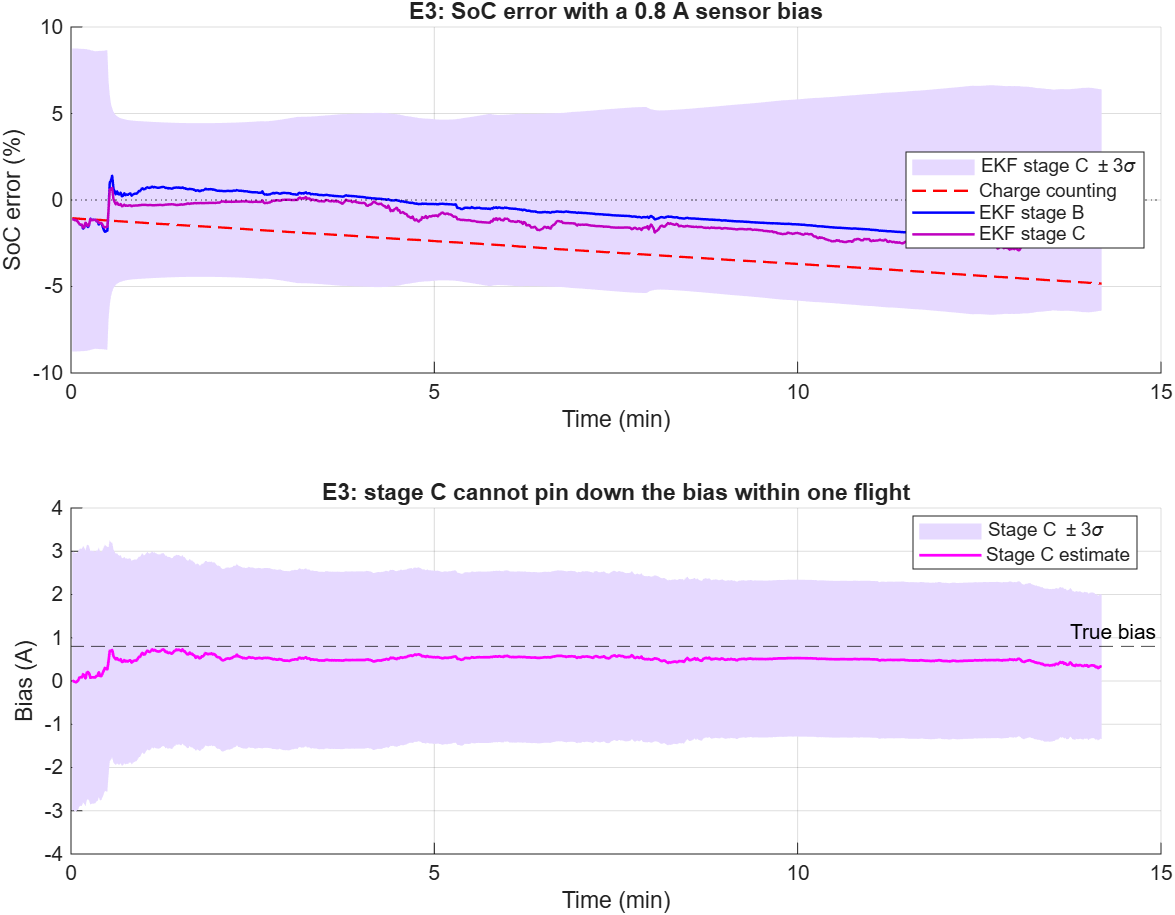
\includegraphics[width=\textwidth]{day4_e3_bias.png}
  \caption{E3, sensor bias 0.8\,A. Top: SoC error of charge counting, stage B and stage C, with the stage-C $\pm 3\sigma$ band. Bottom: stage-C bias estimate with its band. Notice that charge counting drifts steadily while both EKF stages stay within about 3\%, and that the bias estimate settles near 0.5\,A, below the true 0.8\,A, with a band that stays wide: the bias is only partly learned in one flight.}
  \label{fig:r_e3}
\end{figure}

\subsection{E4: Capacity observability (stage C)}\label{sec:r_e4}

In E4 the true battery had aged to 85\% of its rated capacity (4.25\,Ah instead of 5.00\,Ah) and started full, so that it could still complete the short mission. All estimators assumed 5.00\,Ah at the start.

\textbf{Charge counting} ended $+10.20\%$ too high. At landing the true SoC was 9.9\%, below the 10\% reserve, while charge counting believed 20.1\%. Most of this error comes from the capacity: the charge actually drawn, about 3.8\,Ah, is 90\% of 4.25\,Ah but only about 77\% of 5\,Ah.

\textbf{Stage B failed, in the dangerous direction.} Its error grew almost parallel to that of charge counting (Figure~\ref{fig:r_e4}, top), ending at $+8.47\%$. Its band contained the truth only 28\% of the time, and its mean NEES was 44.81, far above 1. Stage~B was therefore confidently wrong, and wrong on the optimistic side: a drone using it would believe it had more charge than it had and would turn back too late. This is the failure predicted by the design check (Section~\ref{sec:m_ekf_choice}). The voltage falls faster than stage~B expects, and stage~B blames the shortfall on its resistance state instead of lowering its SoC.

\textbf{Stage C stayed accurate and honest}: RMSE 0.80\%, final error $+0.17\%$, 100\% inside its band, mean NEES 0.22. Its capacity estimate fell from 5.0\,Ah to about 4.35--4.45\,Ah within about 5\,minutes and ended at 4.45\,Ah, against the true 4.25\,Ah (Figure~\ref{fig:r_e4}, bottom). Its bias estimate ended at $-0.42$\,A, against a true $+0.50$\,A: the wrong sign. The two errors compensate each other. With a measured cruise current of about $15 + 0.5$\,A, the filter's discharge rate \eqref{eq:m_rate} is approximately $(15 + 0.5 + 0.42)/4.45 \approx 3.58$ per hour, against the true $15/4.25 \approx 3.53$ per hour. The rate, which is what the voltage can check, is right to within about 1.5\%, although its two parts are individually wrong. This confirms the observability argument of Section~\ref{sec:m_ekf_choice}.

\begin{figure}[htbp]
  \centering
  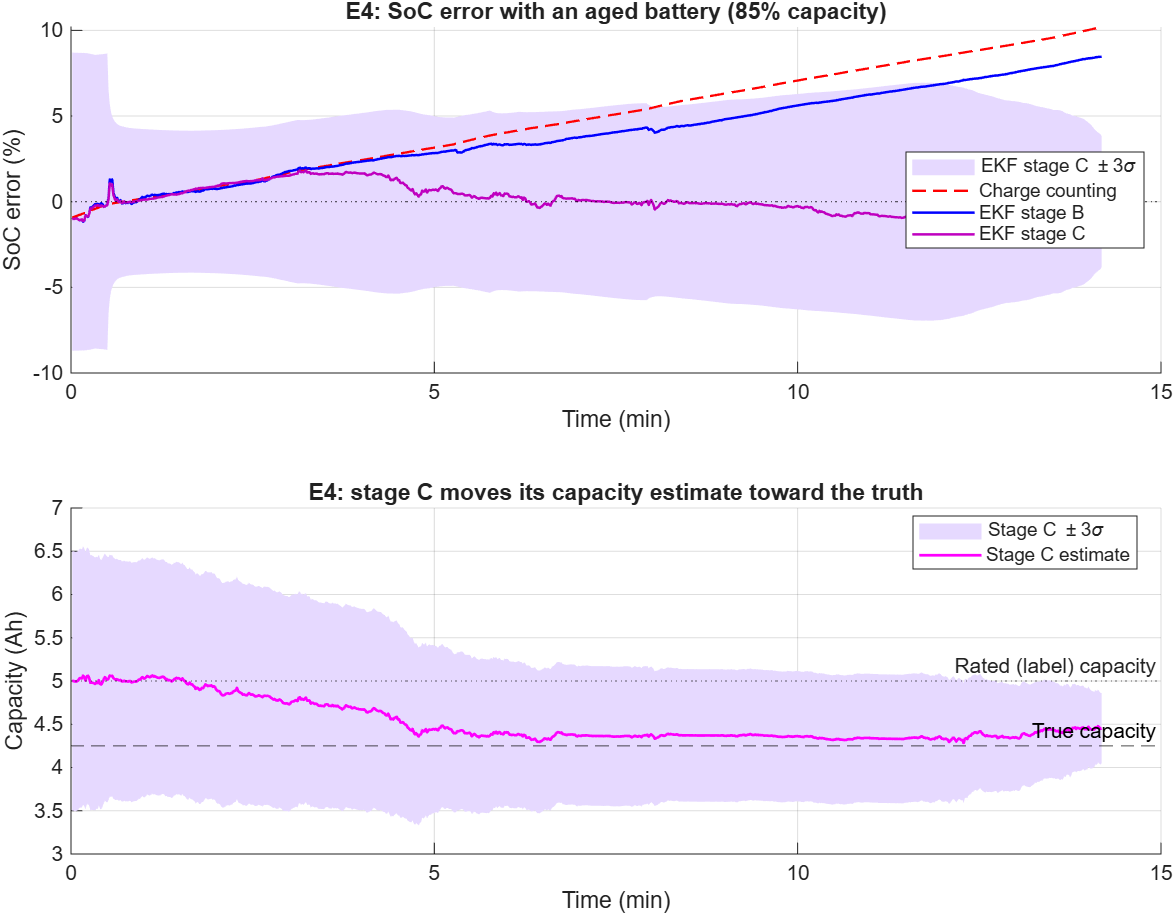
\includegraphics[width=\textwidth]{day4_e4_aged.png}
  \caption{E4, battery aged to 85\% capacity. Top: SoC error of charge counting, stage B and stage C, with the stage-C $\pm 3\sigma$ band. Bottom: stage-C capacity estimate with its band. Notice that stage B's error grows almost as fast as that of charge counting and leaves the band, both overestimating the SoC, while stage C stays near zero as its capacity estimate falls from 5.0 towards the true 4.25\,Ah within about 5 minutes.}
  \label{fig:r_e4}
\end{figure}

\subsection{E5: Tuning Q and R}\label{sec:r_e5}

E5 reran stage~B on the E1 scenario with $Q$ or $R$ scaled by 0.01 or 100 (Table~\ref{tab:r_e5}, Figure~\ref{fig:r_e5}).

\begin{table}[htbp]
  \centering
  \caption{E5: stage B on E1 with different tunings (seed 2).}
  \label{tab:r_e5}
  \small
  \begin{tabular}{@{}lccccc@{}}
    \toprule
    Tuning & RMSE & Final error & Inside $\pm 3\sigma$ & Mean NIS & Mean NEES \\
    \midrule
    $Q{\times}1$, $R{\times}1$ (chosen) & 1.06\% & $-1.92\%$ & 100\% & 0.51  & 2.12 \\
    $Q{\times}0.01$  & 0.67\% & $-1.27\%$ & 94\%  & 0.54  & 2.41 \\
    $Q{\times}100$   & 2.35\% & $-3.92\%$ & 100\% & 0.32  & 0.66 \\
    $R{\times}0.01$  & 2.77\% & $-4.19\%$ & 30\%  & 32.34 & 53.55 \\
    $R{\times}100$   & 1.69\% & $-2.56\%$ & 100\% & 0.01  & 0.52 \\
    \bottomrule
  \end{tabular}
\end{table}

\begin{itemize}
  \item \textbf{$Q{\times}100$:} the filter distrusts its model, so it follows the voltage noise. Its error is jumpy and it is less accurate (RMSE 2.35\%). The band is honest but wider than needed (NIS 0.32).
  \item \textbf{$Q{\times}0.01$:} the filter trusts its model more. In this run it was slightly more accurate (RMSE 0.67\%), but its band held the truth only 94\% of the time: it has less margin for the model errors it does not know about.
  \item \textbf{$R{\times}0.01$:} the filter believes every wiggle of the voltage. During the first 30\,s, before $R_0$ has been learned at the take-off current step, its SoC error swung down to about $-13\%$ (Figure~\ref{fig:r_e5}). It was badly overconfident: 30\% inside its band, mean NEES 53.55. Its mean NIS of 32.34, far above 1, flags the mistuning clearly.
  \item \textbf{$R{\times}100$:} the filter barely uses the voltage. It is smooth but slower to correct (RMSE 1.69\%), and its band is far too wide (NIS 0.01, NEES 0.52). With the RTH rule, such a band would make the drone turn back needlessly early.
\end{itemize}
The chosen tuning was kept. $Q{\times}0.01$ was slightly more accurate in this single run, but it gave up honesty, and the RTH rule relies on $\sigma_{\text{SoC}}$. E5 also shows what NIS can and cannot detect. It flags a wrongly set $R$ clearly ($32 \gg 1$), because that makes the innovations larger than the filter expects. It cannot flag a biased model: in E1 stage~A had a normal-looking NIS but a biased SoC (Section~\ref{sec:r_e1}).

\begin{figure}[htbp]
  \centering
  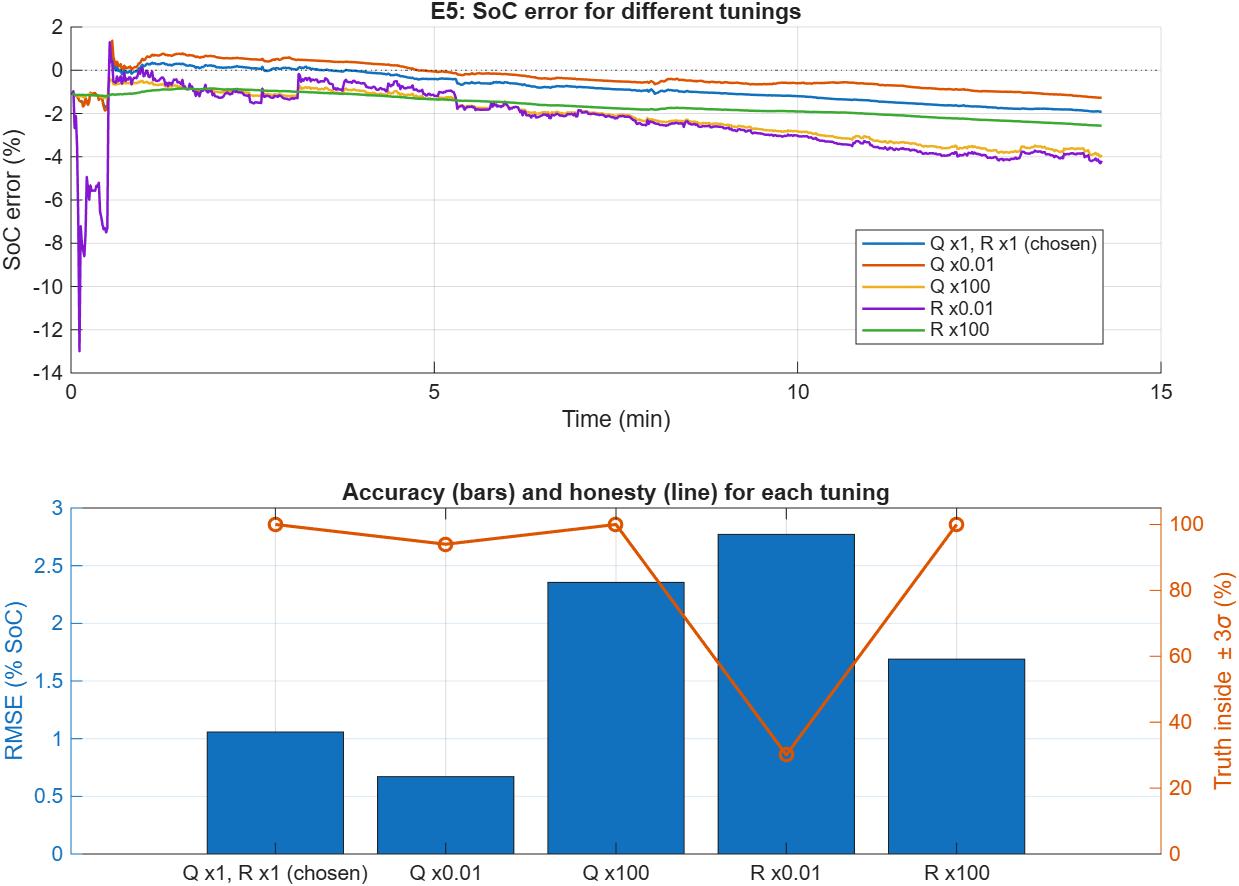
\includegraphics[width=\textwidth]{day4_e5_tuning.png}
  \caption{E5, stage B with five tunings. Top: SoC error over the flight. Bottom: RMSE (bars) and share of time the truth was inside the band (line). Notice the $-13\%$ excursion of $R{\times}0.01$ during take-off and its low band coverage, and that $Q{\times}0.01$ is the most accurate but the only other tuning below 100\% coverage.}
  \label{fig:r_e5}
\end{figure}

\subsection{E6: Model-mismatch stress test}\label{sec:r_e6}

In E6 the true battery's slow RC pair was set to the original, strong value ($R_2 = 4$\,m$\Omega$, $C_2 = 10^5$\,F, $\tau_2 = 400$\,s), about 2.7 times larger in resistance than the default. Table~\ref{tab:r_e6} and Figure~\ref{fig:r_e6} show the results.

\begin{table}[htbp]
  \centering
  \caption{E6: strong model mismatch ($R_2 = 4$\,m$\Omega$), seed 2.}
  \label{tab:r_e6}
  \small
  \begin{tabular}{@{}lccccc@{}}
    \toprule
    Estimator & RMSE & Final error & Inside $\pm 3\sigma$ & Mean NIS & Mean NEES \\
    \midrule
    Charge counting & 2.33\% & $-3.41\%$ & -- & -- & -- \\
    EKF stage A     & 5.11\% & $-7.91\%$ & 2\%  & 0.71 & 406 \\
    EKF stage B     & 2.48\% & $-3.75\%$ & 44\% & 0.53 & 11.8 \\
    EKF stage C     & 4.60\% & $-4.99\%$ & 75\% & 0.52 & 5.56 \\
    \bottomrule
  \end{tabular}
\end{table}

All three filters degraded. The large unmodelled slow drop pulls the voltage down over the flight, and each filter reads part of it as a lower SoC. Stage~A ended at $-7.91\%$ with a NEES of 406. Stage~C drifted to about $-8\%$ around 12\,minutes, leaving its own band, and partly recovered to $-4.99\%$ at landing. Stage~B was about as accurate as charge counting, and stages A and C were worse. Charge counting is not affected at all, because the slow RC pair changes only the voltage, not the charge drawn. None of the filters was consistent: the best band, stage~C's, held the truth 75\% of the time. This is the honest limit of the method: when the filter's model is too wrong, the voltage feedback misleads the EKF, and it becomes biased and overconfident. Section~\ref{sec:d_mismatch} discusses remedies.

\begin{figure}[htbp]
  \centering
  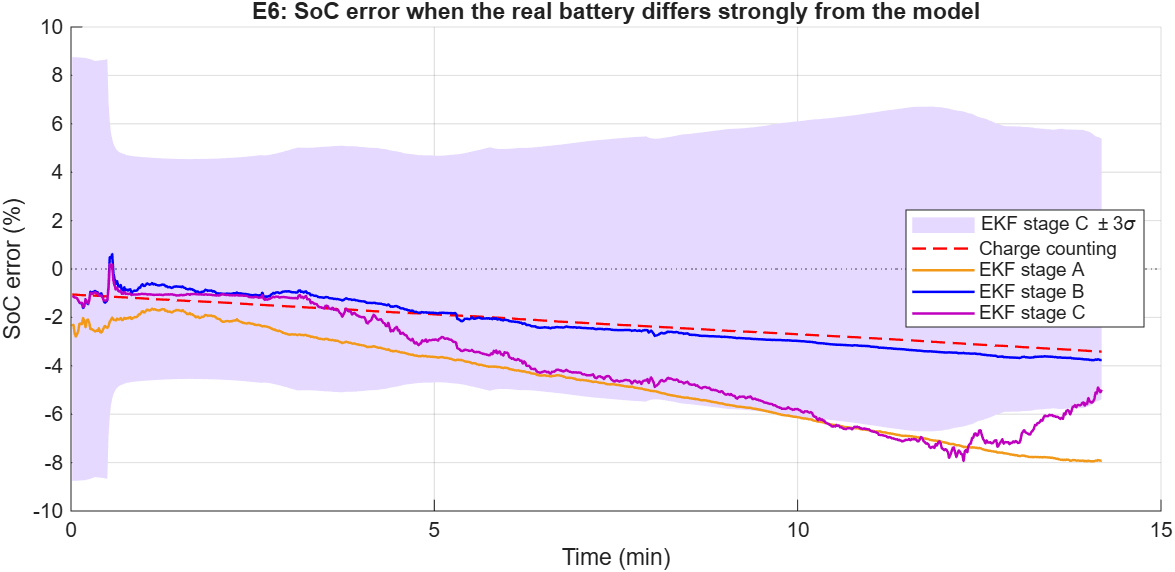
\includegraphics[width=\textwidth]{day4_e6_stress.png}
  \caption{E6, strong model mismatch. SoC error of charge counting and stages A, B and C, with the stage-C $\pm 3\sigma$ band. Notice that all EKF stages drift low, that stage C leaves its band around 12 minutes, and that charge counting, which ignores the voltage, is as good as the best filter here.}
  \label{fig:r_e6}
\end{figure}

\subsection{E7: Flat region of the OCV curve}\label{sec:r_e7}

Figure~\ref{fig:r_e7} plots $\sigma_{\text{SoC}}$ against the true SoC for stages B and C during the E1 flight, after the first minute (the flight runs from about 88\% to 18\%), together with the OCV slope.

\textbf{Stage C} behaves as theory predicts (Section~\ref{sec:bg_gain}). Its uncertainty rises from about 1.5\% to about 2.2\% as the OCV slope falls from about 8 to about 5\,mV per 1\% SoC. The figure contains a sharper test of the cause. Around 65--70\% SoC the OCV slope has a local bump (to about 8.3\,mV per 1\%), and exactly there stage~C's $\sigma_{\text{SoC}}$ dips briefly, from about 1.67\% to about 1.55\%. The uncertainty tracks the slope, not merely the time since take-off: where the voltage says more about the SoC, the filter becomes more certain.

\textbf{Stage B} behaves differently: its uncertainty falls steadily from about 0.95\% to about 0.70\%. Stage~B's only parameter is $R_0$, and the information it collects about $R_0$ at every current change keeps reducing the SoC uncertainty, which masks the flat-region effect. Both behaviours are reported because they show that the stated uncertainty depends on the whole filter structure, not on the OCV curve alone. For the RTH rule, stage~C's behaviour is the desirable one: it becomes more cautious exactly where the voltage is a weaker clue.

\begin{figure}[htbp]
  \centering
  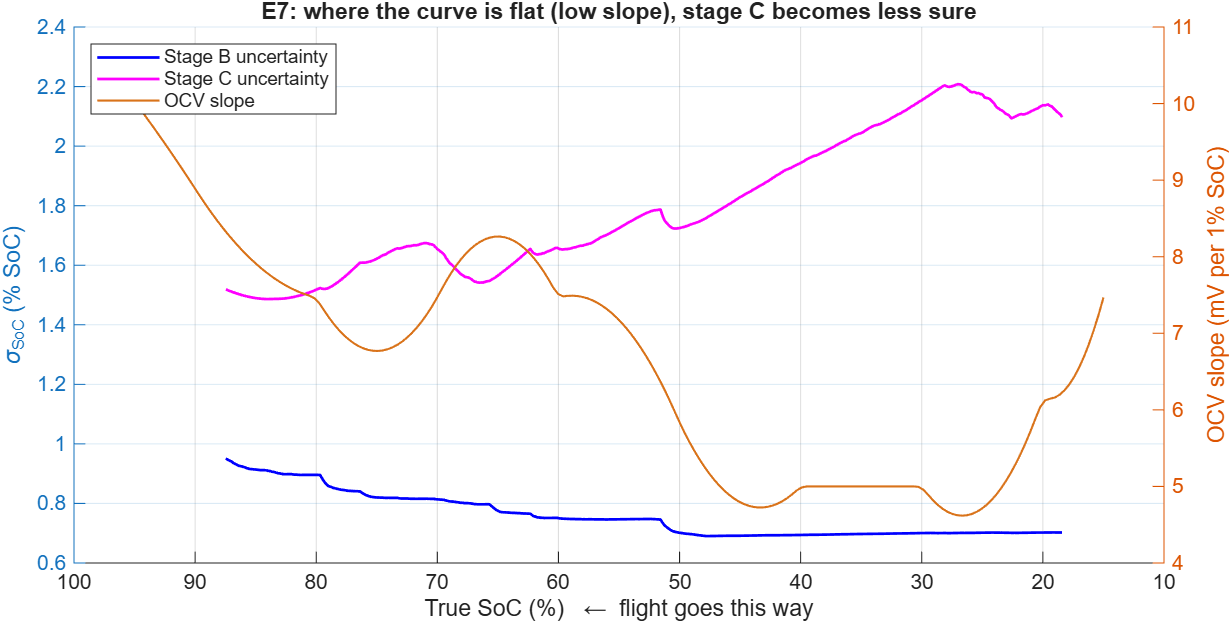
\includegraphics[width=\textwidth]{day4_e7_flat_ocv.png}
  \caption{E7: SoC uncertainty $\sigma_{\text{SoC}}$ of stages B and C against the true SoC (the flight runs from left to right), with the OCV slope on the right axis. Notice that stage C's uncertainty grows as the slope falls, and dips briefly around 65--70\% SoC exactly where the slope has a local bump; stage B's uncertainty falls steadily instead.}
  \label{fig:r_e7}
\end{figure}

\subsection{E8: Comparison of filter stages}\label{sec:r_e8}

E8 flew each of five scenarios with 20 seeds and all three stages, 300 flights in total, in about 20\,s of MATLAB time. Table~\ref{tab:r_e8} gives the mean RMSE and the band coverage, Table~\ref{tab:r_e8_extra} the mean final error and the mean NEES, and Figure~\ref{fig:r_e8} shows the RMSE and coverage graphically.

\begin{table}[htbp]
  \centering
  \caption[E8: mean SoC RMSE and band coverage.]{E8: mean SoC RMSE over 20 flights per scenario, with the share of time the truth was inside the filter's $\pm 3\sigma$ band in brackets.}
  \label{tab:r_e8}
  \small
  \begin{tabular}{@{}lcccc@{}}
    \toprule
    Scenario & Charge counting & Stage A & Stage B & Stage C \\
    \midrule
    E1 Nominal          & 1.83\%  & 2.46\% (16\%) & 1.03\% (100\%) & 1.41\% (100\%) \\
    E2 Wrong start      & 13.84\% & 2.47\% (17\%) & 1.64\% (100\%) & 1.80\% (100\%) \\
    E3 Bias 0.8\,A      & 2.64\%  & 2.31\% (22\%) & 1.27\% (91\%)  & 1.24\% (100\%) \\
    E4 Aged battery     & 6.17\%  & 1.39\% (46\%) & 4.72\% (27\%)  & 1.03\% (100\%) \\
    E6 Strong mismatch  & 1.83\%  & 5.10\% (6\%)  & 2.37\% (50\%)  & 4.16\% (83\%) \\
    \bottomrule
  \end{tabular}
\end{table}

\begin{table}[htbp]
  \centering
  \caption[E8: mean final error and mean NEES.]{E8: mean final SoC error at landing, and mean NEES on the SoC in brackets (about 1 for an honest filter), over 20 flights per scenario (from \texttt{e8\_summary.csv}).}
  \label{tab:r_e8_extra}
  \small
  \begin{tabular}{@{}lcccc@{}}
    \toprule
    Scenario & Charge counting & Stage A & Stage B & Stage C \\
    \midrule
    E1 Nominal          & $-2.87\%$  & $-3.79\%$ (91.5)  & $-1.82\%$ (1.95) & $-1.87\%$ (0.56) \\
    E2 Wrong start      & $+12.65\%$ & $-2.39\%$ (92.9)  & $-0.58\%$ (1.32) & $+0.08\%$ (0.46) \\
    E3 Bias 0.8\,A      & $-4.29\%$  & $-3.78\%$ (83.0)  & $-2.38\%$ (2.91) & $-1.67\%$ (0.43) \\
    E4 Aged battery     & $+10.69\%$ & $+1.91\%$ (30.2)  & $+8.34\%$ (45.6) & $+0.16\%$ (0.40) \\
    E6 Strong mismatch  & $-2.87\%$  & $-7.82\%$ (403.8) & $-3.69\%$ (10.8) & $-4.69\%$ (4.69) \\
    \bottomrule
  \end{tabular}
\end{table}

\begin{figure}[htbp]
  \centering
  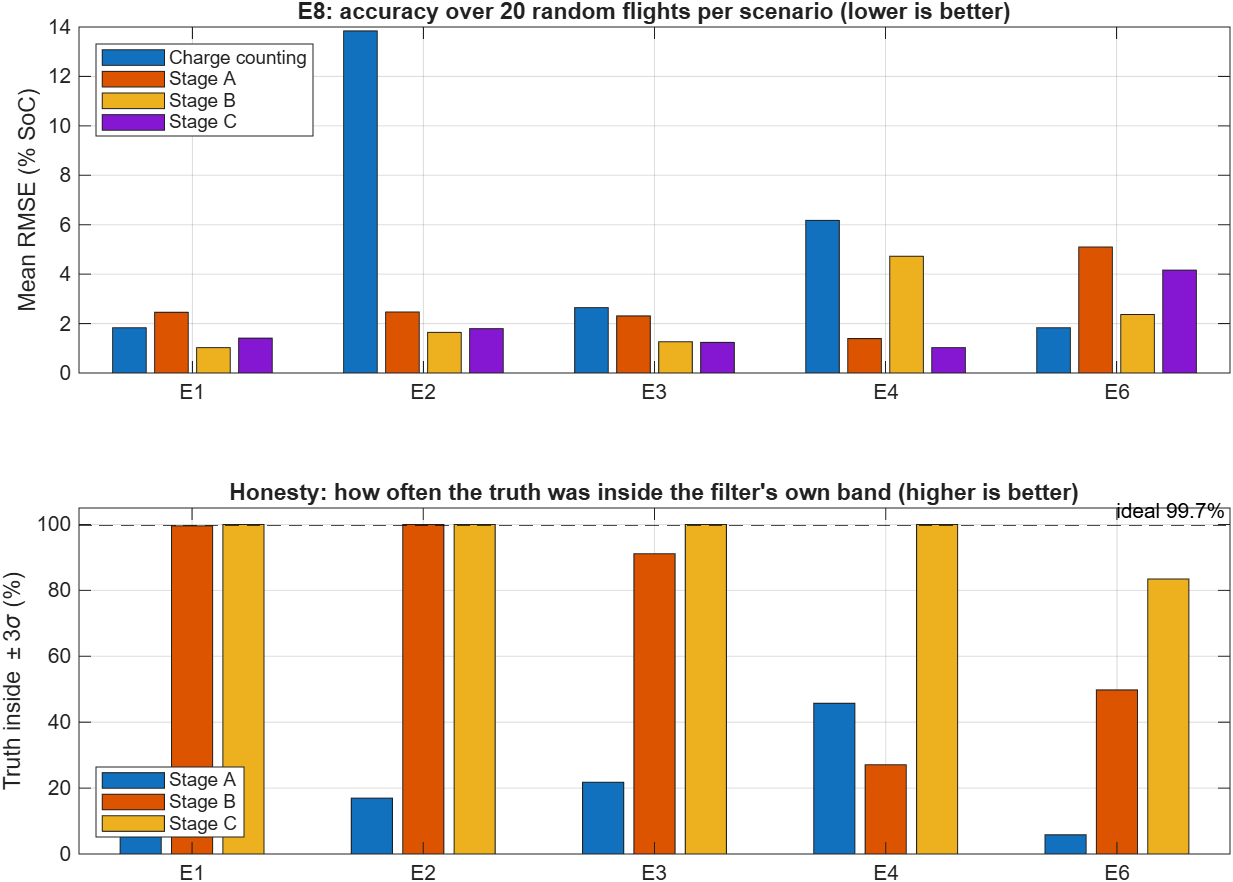
\includegraphics[width=\textwidth]{day4_e8_summary.png}
  \caption{E8, 20 flights per scenario. Top: mean SoC RMSE of charge counting and stages A, B and C. Bottom: share of time the truth was inside each filter's $\pm 3\sigma$ band, with the ideal 99.7\% marked. Notice that stage C is the only filter that reaches about 100\% coverage in every scenario except the strong mismatch E6, and that stage B's accuracy and coverage both collapse on the aged battery (E4).}
  \label{fig:r_e8}
\end{figure}

The 20-flight averages confirm the single runs and the early Python tests (Section~\ref{sec:m_ekf_choice}).
\begin{itemize}
  \item \textbf{Stage C is the only consistent filter in E1--E4.} Its band held the truth 100\% of the time in all four scenarios, with mean RMSE between 1.03\% and 1.80\%. Its mean NEES (0.40--0.56) is below 1, so it is slightly cautious, in line with its mean NIS of about 0.49.
  \item \textbf{Stage B is the most accurate on a healthy battery} (1.03\% in E1, 1.64\% in E2), but it fails on the aged battery: 4.72\% RMSE, 27\% coverage, a mean final error of $+8.34\%$ (optimistic) and a mean NEES of 45.6. It is also slightly overconfident with the larger bias (91\% coverage in E3).
  \item \textbf{Stage A is never consistent} (6--46\% coverage, NEES 30--404), although its mean NIS stayed around 0.5--1.1. In E4 its accuracy looks good (1.39\%), but this is probably a coincidence of two errors cancelling: its resistance error pulls the SoC low (as in E1, final $-3.79\%$), while the aged capacity pushes it high.
  \item \textbf{Charge counting} is badly affected by a wrong start (13.84\%) and an aged battery (6.17\%, optimistic). In E6 it gives exactly the same result as in E1, because the slow RC pair affects only the voltage.
  \item \textbf{Under strong mismatch (E6) no filter is consistent} (at most 83\% coverage), and the most accurate filter there (stage~B, 2.37\%) does not beat charge counting (1.83\%).
\end{itemize}

\textbf{Conclusion for the decision filter.} Stage~C is the only filter whose uncertainty stayed honest in all of E1--E4, with an RMSE of 1.0--1.8\%. Stage~B is the most accurate on a healthy battery, but on an aged battery it becomes confidently optimistic, which is the dangerous failure for an RTH decision. The MATLAB results therefore confirm the design choice of Section~\ref{sec:m_ekf_choice}: stage~C provides the SoC estimate and $\sigma_{\text{SoC}}$ for the RTH rule. The strong-mismatch case E6 remains a stated limitation (Section~\ref{sec:d_limitations}).

%--------------------------------------------------------------------------------------------------
\section{Return-to-home decisions on a single flight}\label{sec:r_single_rth}
%--------------------------------------------------------------------------------------------------

The demonstration mission (Section~\ref{sec:m_experiments}) was flown on the long route with each of the four policies under the same difficult conditions: start at 95\%, a battery aged to 85\% of its capacity, a current sensor reading 0.5\,A low ($b = -0.5$\,A), a 10\% headwind, and noise seed~7. Table~\ref{tab:r_demo} summarises the outcomes, and Figures~\ref{fig:r_demo_decision} and~\ref{fig:r_demo_map} show how they came about.

\begin{table}[htbp]
  \centering
  \caption{Demonstration mission: outcome under each policy.}
  \label{tab:r_demo}
  \small
  \begin{tabular}{@{}lcccc@{}}
    \toprule
    Policy & Turn-back & Deliveries & True SoC at landing & Outcome \\
    \midrule
    A. Voltage threshold (3.5\,V) & 6.4\,min & 1 & 11.7\% & Safe \\
    B. Charge counting           & 8.2\,min & 2 & 0.0\%  & Battery died \\
    C. EKF estimate only         & 6.4\,min & 1 & 11.9\% & Safe \\
    D. EKF risk-aware (95\%)     & 5.9\,min & 1 & 17.8\% & Safe \\
    \bottomrule
  \end{tabular}
\end{table}

\begin{figure}[htbp]
  \centering
  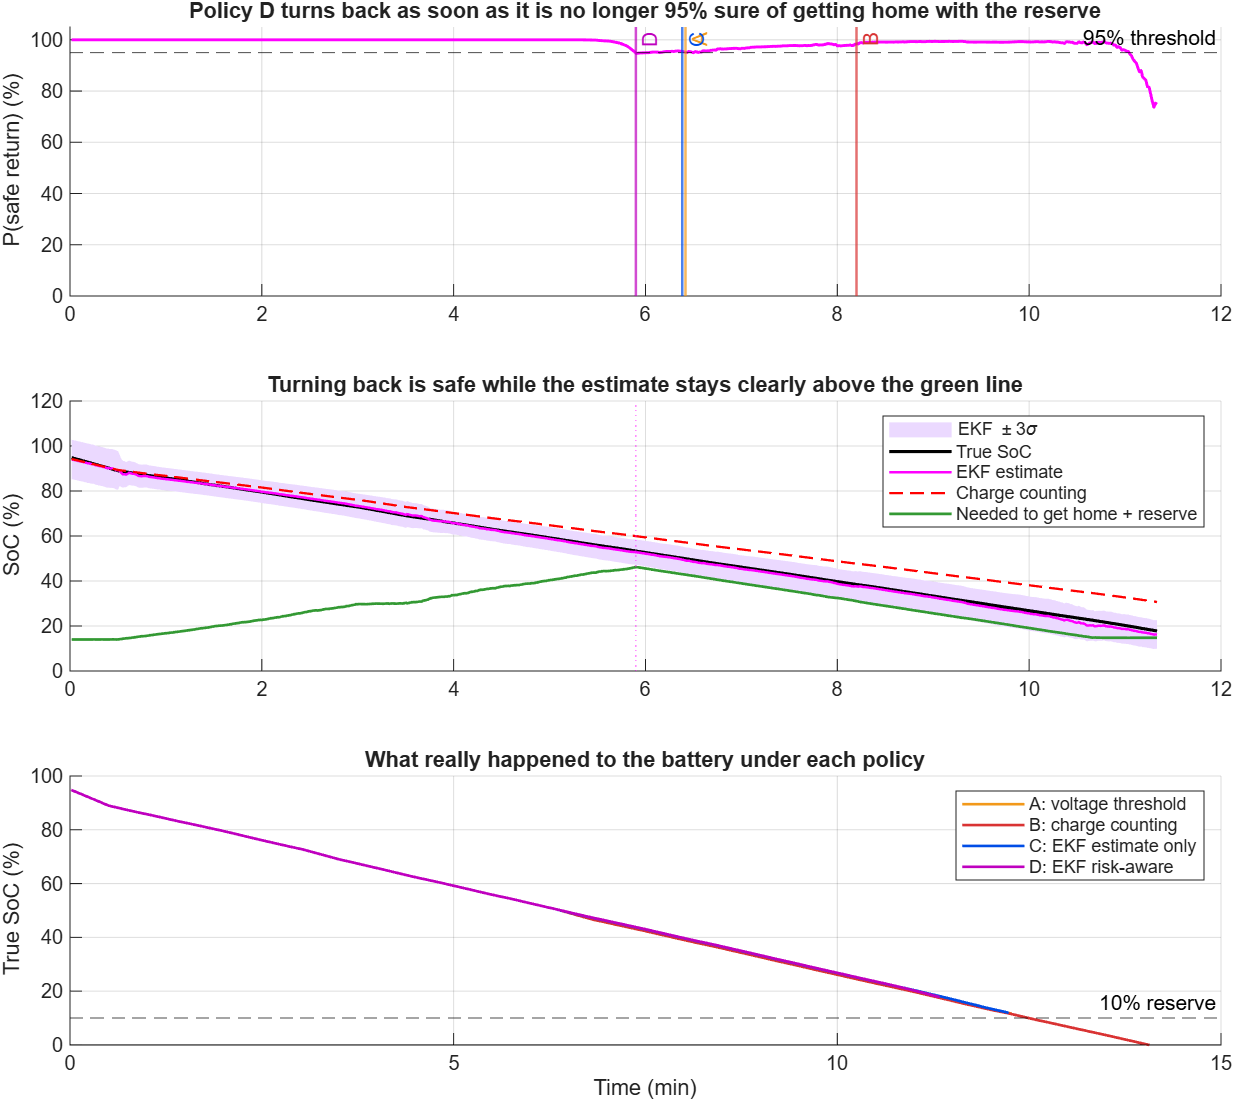
\includegraphics[width=\textwidth]{day5_demo_decision.png}
  \caption{Demonstration mission. Top: $P_{\text{safe}}$ during policy D's flight, with the turn-back time of each policy marked. Middle: true SoC, stage-C estimate with its $\pm 3\sigma$ band, charge counting, and the SoC needed to get home plus the reserve (green). Bottom: true SoC under each policy. Notice that D turns back when the lower edge of the EKF band approaches the green line, that charge counting runs well above the truth, and that only B's battery falls through the reserve to zero.}
  \label{fig:r_demo_decision}
\end{figure}

\begin{figure}[htbp]
  \centering
  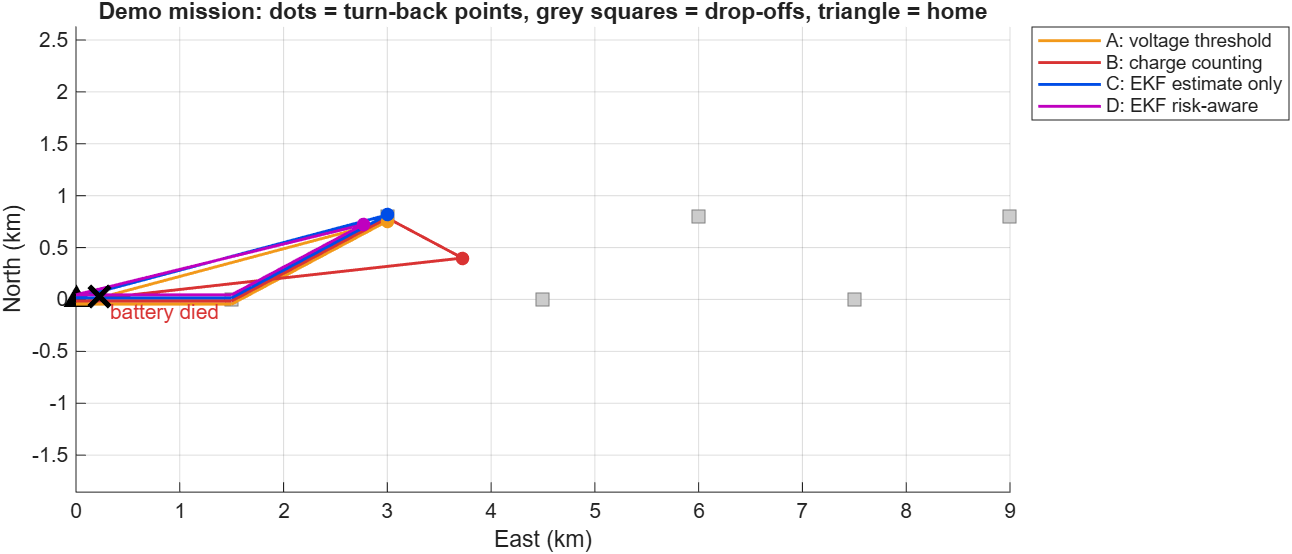
\includegraphics[width=\textwidth]{day5_demo_map.png}
  \caption{Demonstration mission: flight paths and turn-back points (dots) of the four policies; grey squares are drop-offs and the triangle is home. Notice that A, C and D turn back near drop-off 2, while B carries on towards drop-off 3 and its battery dies just short of home.}
  \label{fig:r_demo_map}
\end{figure}

\textbf{The estimators.} In the middle panel of Figure~\ref{fig:r_demo_decision}, the stage-C estimate stays close to the true SoC, inside its band, for the whole flight. Charge counting runs about 7--12\% above the truth, and the gap grows. Both conditions of this mission make it optimistic: the aged battery empties faster than the rated 5\,Ah suggests, and the low-reading sensor hides part of the current drawn. The SoC needed to get home plus the reserve (green) rises as the drone flies away from home and peaks at about 46\% when policy~D turns back.

\textbf{The decisions.}
\begin{itemize}
  \item \textbf{D} kept $P_{\text{safe}}$ near 100\% until about 5.8\,min. It then fell to 95\%, and D turned back at 5.9\,min, on the way to drop-off~2, when the estimate minus its uncertainty met the green line. It landed with 17.8\%, that is 7.8 points above the reserve.
  \item \textbf{C} and \textbf{A} both turned back 0.5\,min later, at 6.4\,min, while hovering at drop-off~2 (Figure~\ref{fig:r_demo_map}). Because a drop counts only once its hover is finished, this drop does not count, and all three safe policies completed one delivery. C, which aims exactly at the reserve, landed at 11.9\%; A landed at 11.7\%. Both kept the reserve, but only just.
  \item \textbf{B} believed the optimistic charge counter. It completed a second delivery, turned back at 8.2\,min on its way to drop-off~3 (about 3.7\,km east), and its battery died about 200\,m short of home. The reserve that the counter promised did not exist.
\end{itemize}

At the very end of policy~D's flight, $P_{\text{safe}}$ drops to about 75\% (Figure~\ref{fig:r_demo_decision}, top). This is an artefact: during the final landing the formula \eqref{eq:m_dsoc_home} still charges the full 40\,s landing cost, although part of the landing is already done. Decisions are made only in cruise and hover, so it has no effect.

%--------------------------------------------------------------------------------------------------
\section{Monte Carlo study}\label{sec:r_mc}
%--------------------------------------------------------------------------------------------------

The four policies flew the same 500 random missions (Table~\ref{tab:m_mc_factors}), with the same conditions and the same sensor noise; the study took about 95\,s of MATLAB time. Table~\ref{tab:r_mc} and Figure~\ref{fig:r_mc} give the results. Deliveries count a drop only once its hover is finished.

\begin{table}[htbp]
  \centering
  \caption[Monte Carlo results over 500 missions.]{Monte Carlo results over 500 missions. Reserve broken: died, or landed below the 10\% reserve. Unused battery: mean true SoC at landing minus the reserve, over the missions that landed (negative means below the reserve on average).}
  \label{tab:r_mc}
  \small
  \setlength{\tabcolsep}{3pt}
  \begin{tabular}{@{}lccccc@{}}
    \toprule
    Policy & Died & Reserve broken & Unused battery & Deliveries & Died, aged only \\
    \midrule
    A. Voltage (3.5\,V)          & 9.2\%  & 32.2\% & 8.0\%    & 0.85 & 10.0\% \\
    B. Charge counting           & 30.4\% & 90.2\% & $-4.1\%$ & 1.56 & 58.2\% \\
    C. EKF estimate             & 0.0\%  & 38.0\% & 0.6\%    & 1.32 & 0.0\% \\
    D. EKF risk-aware (95\%)     & 0.0\%  & 2.8\%  & 6.1\%    & 1.16 & 0.0\% \\
    \bottomrule
  \end{tabular}
\end{table}

\begin{figure}[htbp]
  \centering
  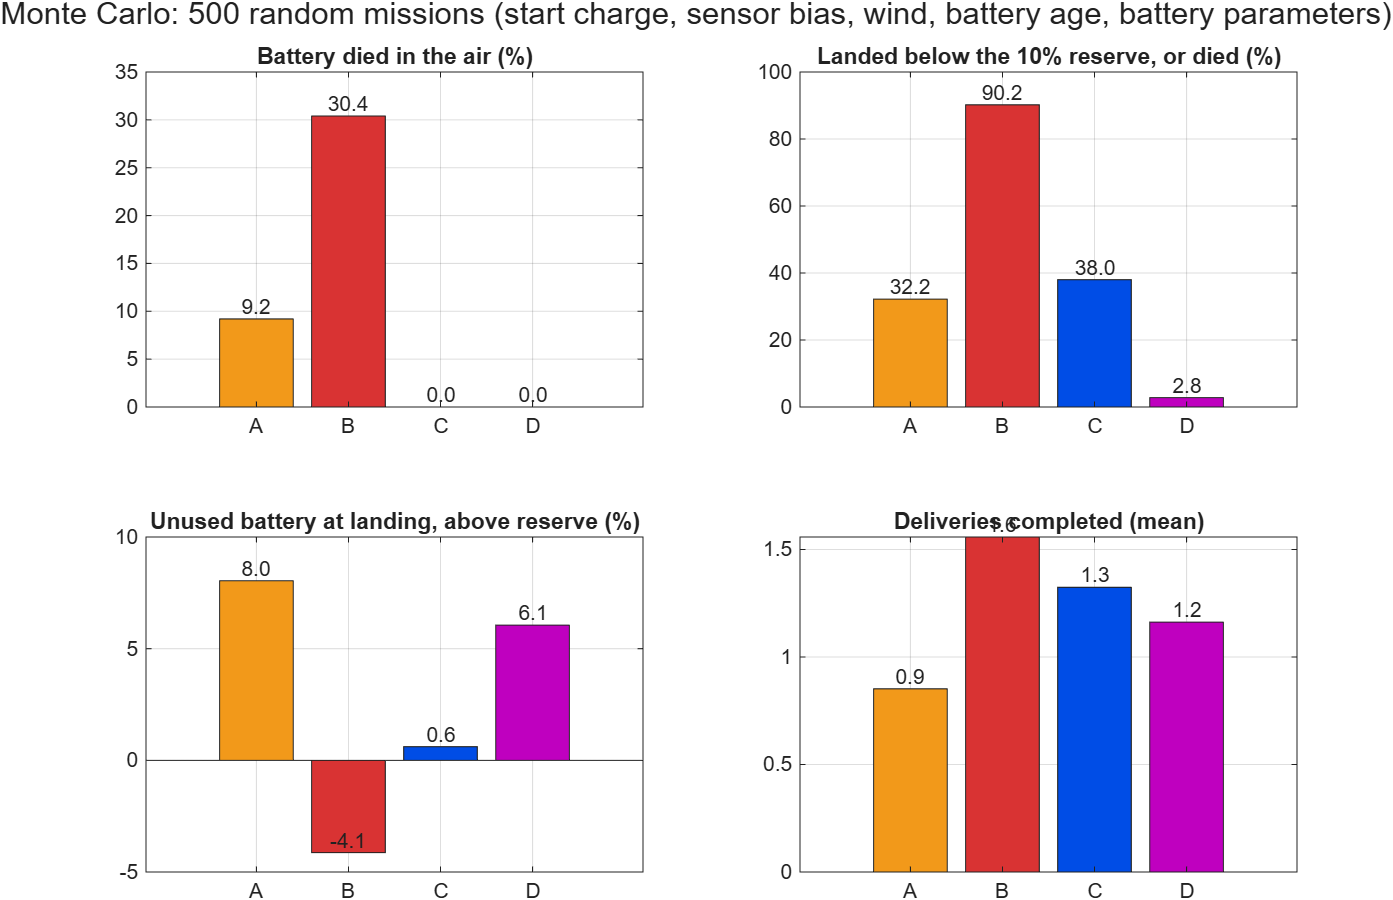
\includegraphics[width=\textwidth]{day5_monte_carlo.png}
  \caption{Monte Carlo study, 500 missions. Share of missions in which the battery died (top left) or the reserve was broken (top right), mean unused battery above the reserve (bottom left), and mean deliveries (bottom right), for each policy. Notice that only D combines zero deaths with a low breach rate, and that B's extra deliveries come with a 30\% death rate.}
  \label{fig:r_mc}
\end{figure}

The aged-battery column covers the 239 missions in which the true capacity was below 90\% of rated.

\textbf{D, the risk-aware rule, is the only policy that is both safe and calibrated.} It had no deaths and broke the reserve in 2.8\% of missions, inside its promise of at most 5\% (Section~\ref{sec:m_rth_prob}). The breach rate is lower than the promise, so the rule is slightly conservative. This matches the finding of E8 that stage~C's uncertainty is slightly larger than necessary (mean NIS about 0.5, mean NEES below 1, Section~\ref{sec:r_e8}). The price is 6.1\% unused battery and 1.16 deliveries per mission.

\textbf{C uses the same filter but ignores its uncertainty.} It also had no deaths, because the stage-C estimate is accurate, but it broke the reserve in 38\% of missions, and its landings sat on average only 0.6 points above the reserve. C turns back when the estimated margin reaches zero, so it aims exactly at the reserve: whenever the estimate or the trip cost is slightly optimistic, the drone lands slightly below it. With unbiased errors this would happen in about half of the missions. The difference between C and D is therefore not the estimator but what is done with its uncertainty.

\textbf{B, charge counting, is dangerous.} The battery died in 30.4\% of all missions and in 58.2\% of the aged-battery missions, and the reserve was broken in 90.2\%. On average it landed below the reserve ($-4.1\%$). Charge counting with the rated capacity is optimistic for an aged battery and for a sensor that reads low, and nothing in it notices. B also "completed" the most deliveries (1.56), but only because it flew on recklessly.

\textbf{A, the voltage threshold, is neither safe nor efficient at 3.5\,V.} It died in 9.2\% of missions and broke the reserve in 32.2\%, while leaving on average 8.0\% of the battery unused, more than D, and completing only 0.85 deliveries. A voltage threshold ignores how far from home the drone is: the same voltage can be plenty close to home and too little far away. Section~\ref{sec:r_sweep} shows that changing the threshold only trades one problem for the other.

\textbf{Estimator accuracy over the Monte Carlo missions.} Over the 500 policy-D flights, which are longer than the flights of E1--E8 and include random battery parameters, the stage-C EKF had a mean SoC RMSE of 1.31\%, against 3.35\% for charge counting, and the true SoC was inside its $\pm 3\sigma$ band 100\% of the time. This agrees with E8 (Table~\ref{tab:r_e8}) and confirms that the uncertainty passed to the decision rule was honest.

%--------------------------------------------------------------------------------------------------
\section{Risk-threshold sweep}\label{sec:r_sweep}
%--------------------------------------------------------------------------------------------------

Policies D and A were rerun on the first 200 Monte Carlo missions with a range of thresholds (Table~\ref{tab:r_sweep}, Figure~\ref{fig:r_tradeoff}).

\begin{table}[htbp]
  \centering
  \caption{Threshold sweep over the first 200 missions. For policy D the promised maximum breach rate, $1 - p^{\ast}$, is given in brackets.}
  \label{tab:r_sweep}
  \small
  \begin{tabular}{@{}llcccc@{}}
    \toprule
    Policy & Threshold & Died & Reserve broken & Unused battery & Deliveries \\
    \midrule
    D & $p^{\ast} = 80\%$   & 0\% & 9.5\% ($\leq 20\%$)  & 3.6\%  & 1.27 \\
      & $p^{\ast} = 90\%$   & 0\% & 4.0\% ($\leq 10\%$)  & 5.0\%  & 1.22 \\
      & $p^{\ast} = 95\%$   & 0\% & 2.0\% ($\leq 5\%$)   & 6.1\%  & 1.18 \\
      & $p^{\ast} = 99\%$   & 0\% & 0.0\% ($\leq 1\%$)   & 8.2\%  & 1.15 \\
      & $p^{\ast} = 99.9\%$ & 0\% & 0.0\% ($\leq 0.1\%$) & 10.4\% & 1.11 \\
    \midrule
    A & $V_{\text{thr}} = 3.40$\,V & 96.0\% & 100.0\% & $-7.9\%$ & 1.88 \\
      & $V_{\text{thr}} = 3.45$\,V & 56.5\% & 84.0\%  & $-1.0\%$ & 1.41 \\
      & $V_{\text{thr}} = 3.50$\,V & 11.0\% & 35.0\%  & 7.5\%    & 0.89 \\
      & $V_{\text{thr}} = 3.55$\,V & 0.5\%  & 3.0\%   & 17.9\%   & 0.56 \\
      & $V_{\text{thr}} = 3.60$\,V & 0\%    & 0\%     & 28.7\%   & 0.36 \\
    \bottomrule
  \end{tabular}
\end{table}

\begin{figure}[htbp]
  \centering
  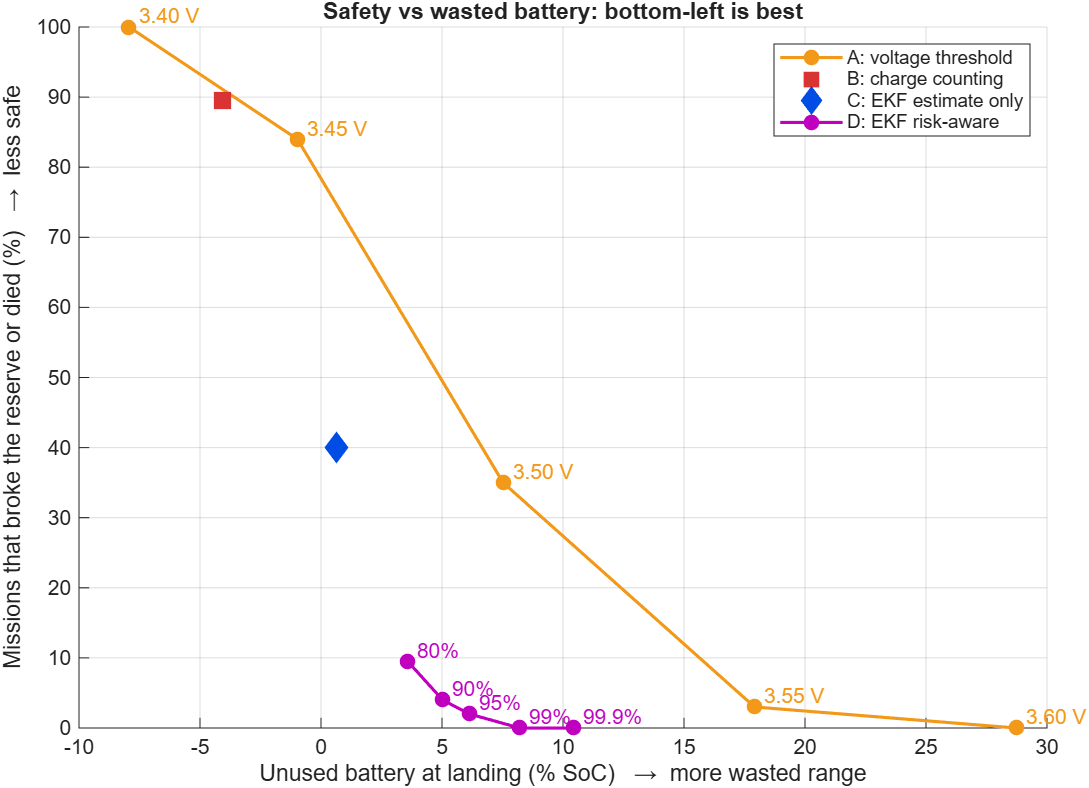
\includegraphics[width=0.9\textwidth]{day5_tradeoff.png}
  \caption{Safety against wasted battery over 200 missions: share of missions that broke the reserve or died, against the mean unused battery, for each threshold of policies A and D, with B and C as single points. Bottom-left is best. Notice that D's curve lies far below A's at every level of unused battery, and that B and C sit far above it.}
  \label{fig:r_tradeoff}
\end{figure}

\textbf{D keeps its promise at every threshold.} No mission died at any threshold, and the breach rate was always within the promise $1 - p^{\ast}$: 9.5\% against at most 20\%, 4.0\% against 10\%, 2.0\% against 5\%, and none at 99\% and 99.9\%. At the three lower thresholds the breach rate was about half the promise, which again shows a slightly conservative uncertainty. With 200 missions the smallest non-zero breach rate that can be observed is 0.5\%, so the 99.9\% promise ($\leq 0.1\%$) is not contradicted, but it cannot be confirmed either.

\textbf{No voltage threshold works.} Low thresholds kill the drone (96\% died at 3.40\,V, 56.5\% at 3.45\,V). To reach D's level of safety, A needs 3.55\,V (3.0\% broken), but then it wastes 17.9\% of the battery, about three times D's 6.1\% at 95\%, and completes only 0.56 deliveries, about half of D's 1.18. In Figure~\ref{fig:r_tradeoff}, for every voltage threshold that keeps the breach rate below that of policy C, there is a D threshold that is at least as safe and less wasteful. The only A points with less unused battery than D are those that land below the reserve on average. B and C, which have no threshold to tune, sit far above D's curve.

\textbf{The price of safety.} Moving D from 90\% to 99\% raised the unused battery from 5.0\% to 8.2\% and cut the deliveries from 1.22 to 1.15; moving from 99\% to 99.9\% cost a further 2.2 points of battery and 0.04 deliveries. Each extra ``nine'' therefore costs a few percent of the battery and a few hundredths of a delivery per mission. The curve lets an operator choose the point that suits the risk they can accept; 95\% is a reasonable default, with a breach rate of about 2--3\% and about 6\% unused battery.
